\documentclass[11pt]{article}
\usepackage[utf8]{inputenc}
\usepackage[T1]{fontenc}
\usepackage{amsmath,amssymb,graphicx,url,tabularx,booktabs}
\usepackage[margin=1in]{geometry}
\renewcommand{\thefigure}{S\arabic{figure}}
\renewcommand{\thetable}{S\arabic{table}}
\title{Supplementary Material for ``Oxidation-Budgeted Design of Lead-Free RbGeI3 Solar Cells: Back-Surface-Field Enhancement, Realistic Loss Budgeting and SHAP Sensitivity From SCAPS-1D Optimization to Manufacturing Tolerances, Benchmarked Against CsGeI3''}
\author{Md.\ Abdul Malek Fahim and Hussain Touhid Siddiquee\thanks{Corresponding author: touhidsiddiqueeraj@gmail.com}}
\begin{document}
\maketitle

\section*{S1.\ One-at-a-time sweep details}
Full per-parameter traces for the eleven sequential optimization steps summarized in Section~V.B of the main text.
\subsection*{Effect of absorber layer thickness}
Thickness sets the trade-off between light capture and recombination: a thicker absorber absorbs more photons and lifts J$_{\mathrm{SC}}$, up to the point where the extra volume becomes a recombination liability.
PCE peaks on a 0.7--0.8 $\mu$m plateau (21.21\%) and eases off beyond it as recombination grows. J$_{\mathrm{SC}}$ climbs steadily with thickness, 25.16 to 31.29 mA/cm$^{2}$ --- all below the R\"uhle SQ limit of 32.88 mA/cm$^{2}$ at 1.4 eV --- while V$_{\mathrm{OC}}$ slides from 0.923 to 0.856 V. The 0.7 $\mu$m point, where the two effects balance, is the one we keep.


\begin{figure}[htbp]
\centering
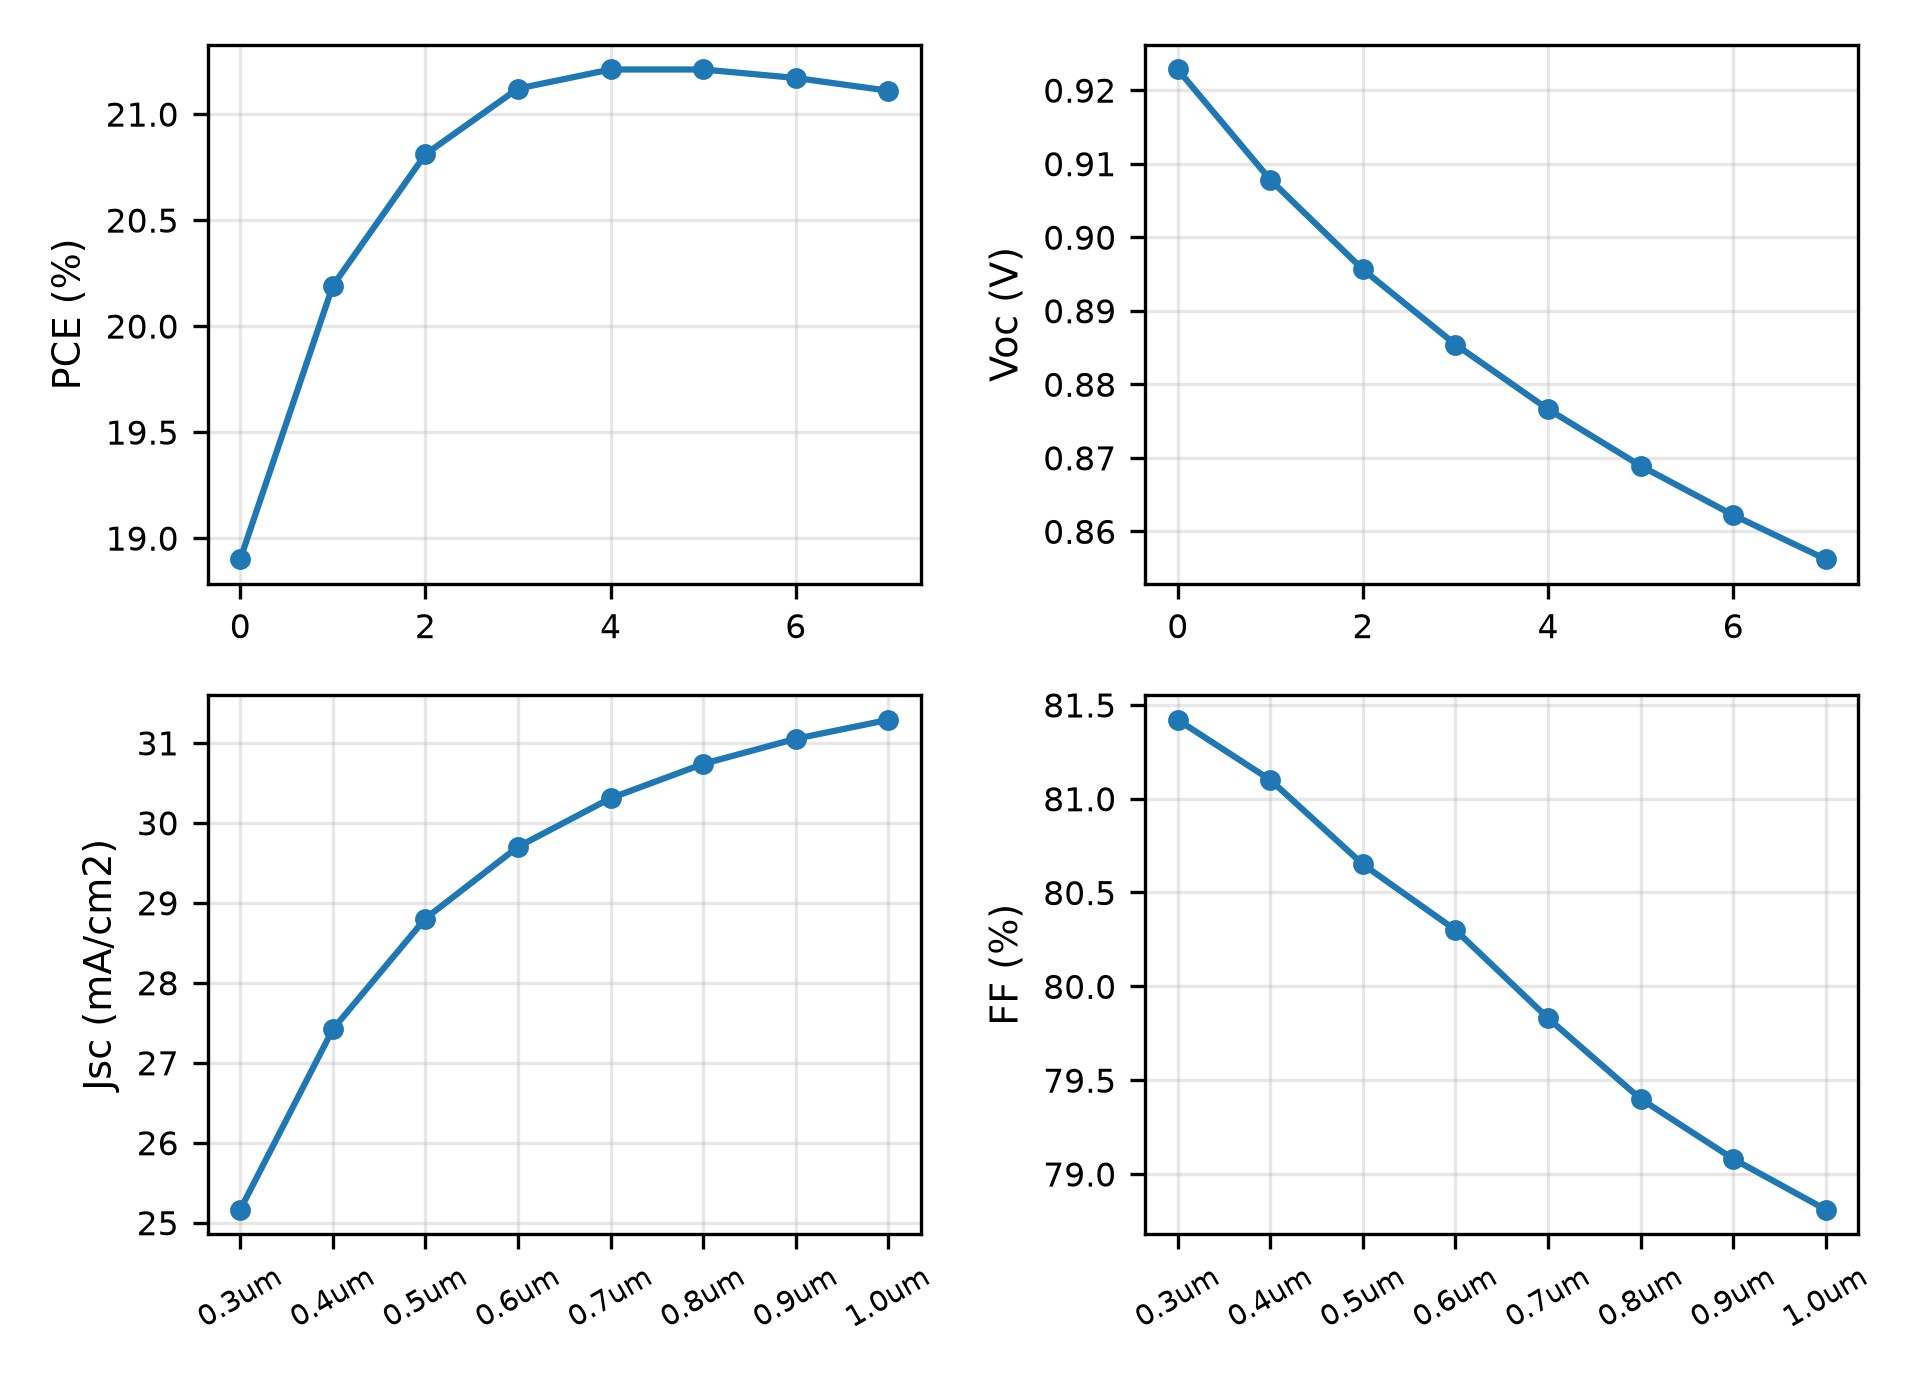
\includegraphics[width=0.85\linewidth]{figs/fig3.png}
\caption{Variation of PCE, V$_{\mathrm{OC}}$, J$_{\mathrm{SC}}$, and FF with RbGeI$_{3}$ absorber thickness. PCE peaks at 0.7 $\mu$m, beyond which recombination losses reduce efficiency.}
\par\vspace{2pt}{\footnotesize\emph{Alt text: Line panels of the photovoltaic parameters against absorber thickness. Efficiency peaks at 0.7 micrometres and falls beyond it as recombination losses grow.}}\par
\end{figure}

\subsection*{Effect of absorber dielectric constant}
The dielectric constant shows a weak monotonic rise (23.05\% at 10, 22.90 at 12, 23.19 at 15, 25.22 at 18, 25.25 at 21, 25.27 at 23.1, extending to 25.35 at 35), carried by V$_{\mathrm{OC}}$ at flat J$_{\mathrm{SC}}$. Since $\epsilon_{r}$ cannot be ordered from a supplier, it is pinned at the prior mid-range value 15 with the full trace disclosed, rather than carried at a grid edge; the pinning cost is stated in the main text.


\begin{figure}[htbp]
\centering
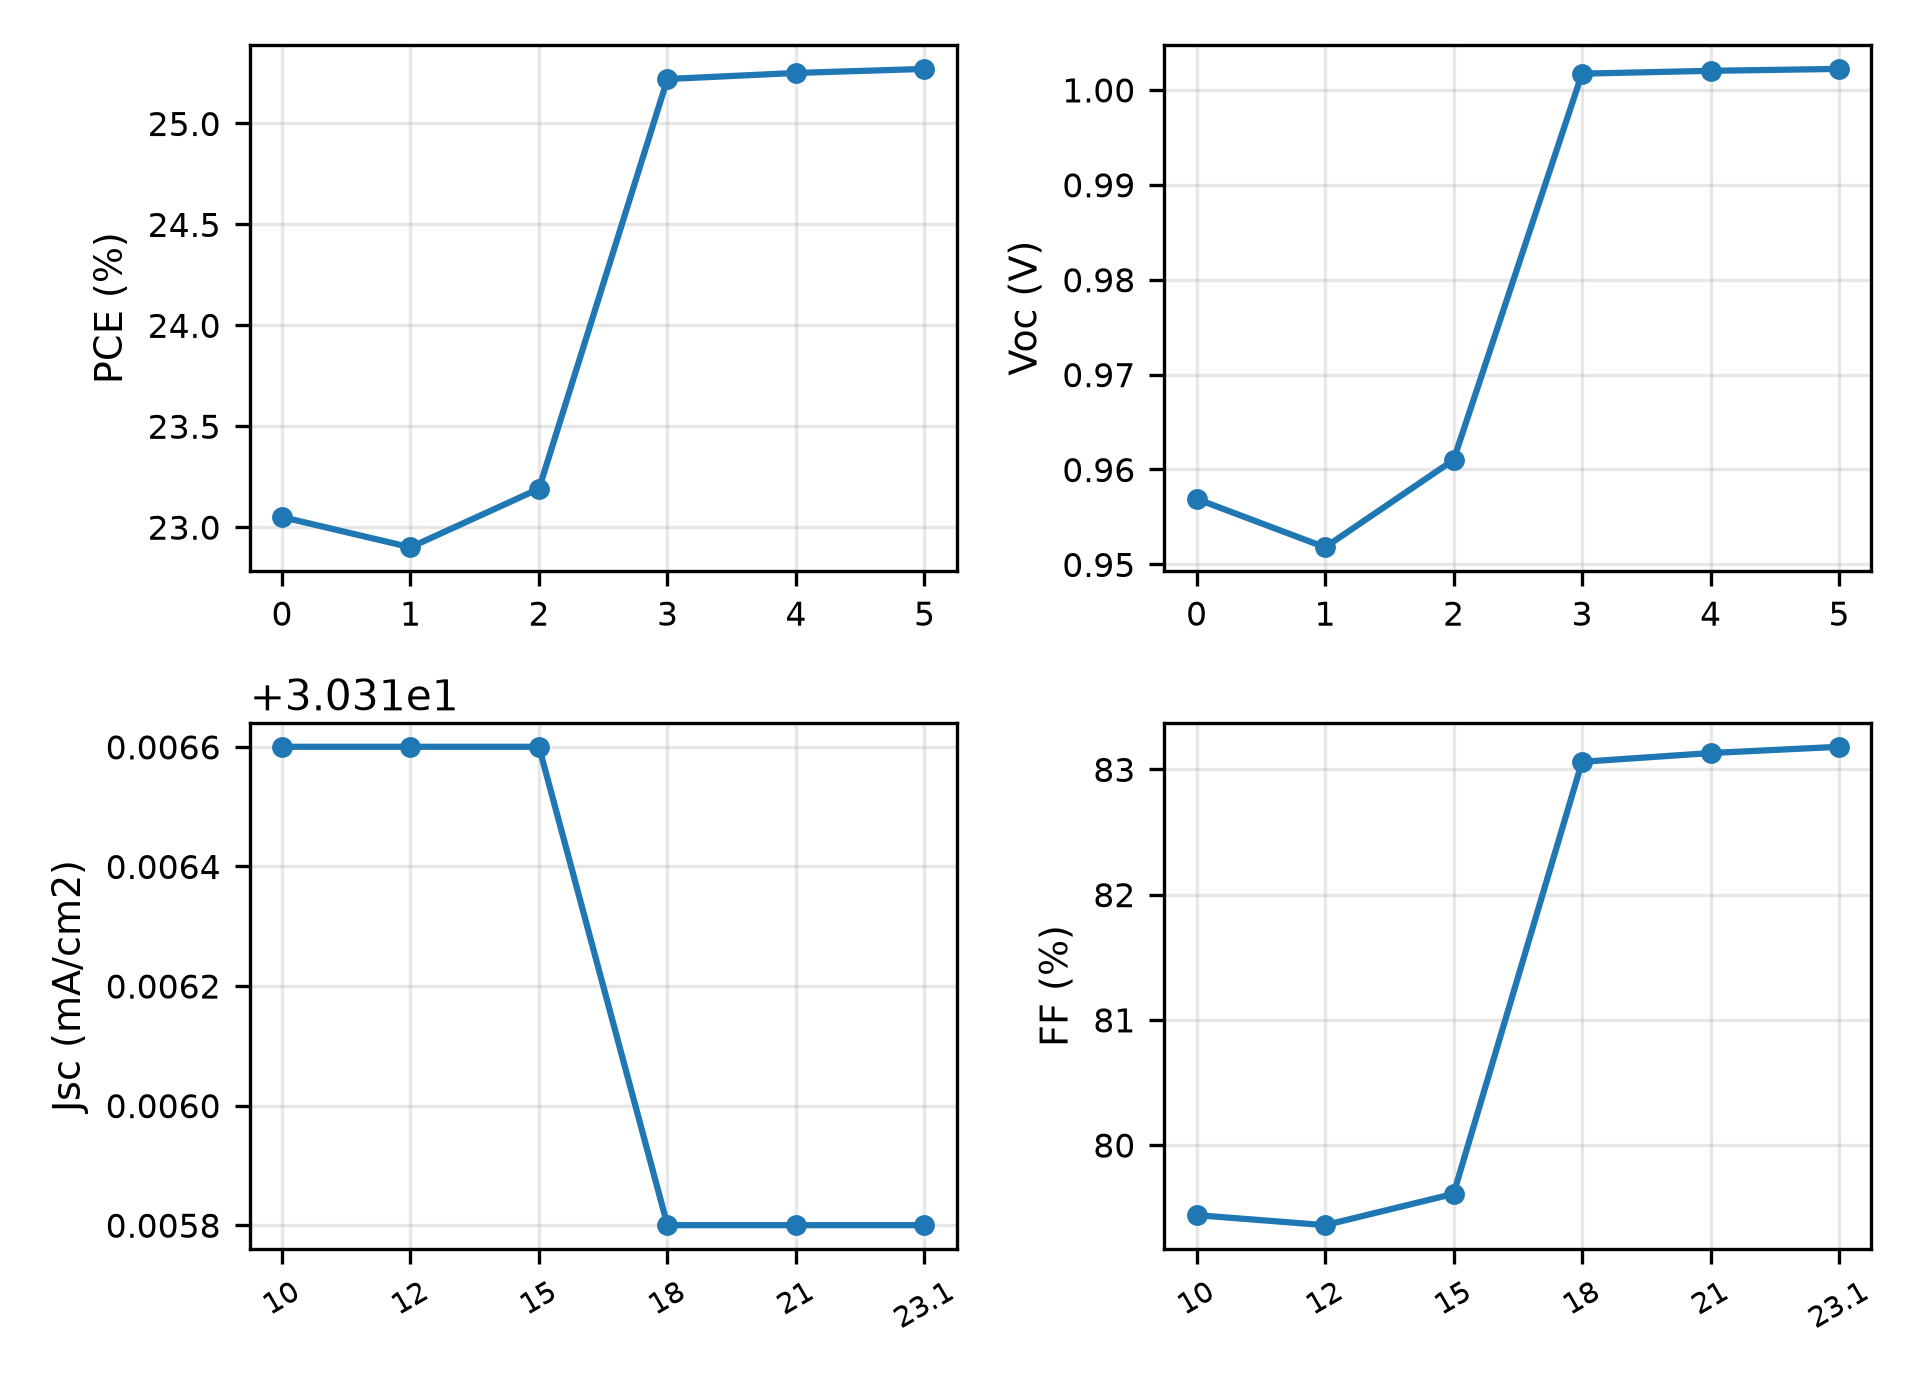
\includegraphics[width=0.85\linewidth]{figs/fig5.png}
\caption{Variation of PCE, V$_{\mathrm{OC}}$, J$_{\mathrm{SC}}$, and FF with RbGeI$_{3}$ absorber dielectric constant. The performance is essentially insensitive to $\epsilon$r across the investigated range; $\epsilon$r = 15 is used in the final device.}
\par\vspace{2pt}{\footnotesize\emph{Alt text: Line panels of the photovoltaic parameters against absorber thickness. Efficiency peaks at 0.7 micrometres and falls beyond it as recombination losses grow.}}\par
\end{figure}

\subsection*{Effect of absorber electron affinity}
Electron affinity lines up the energy bands between adjacent layers and so controls extraction of the charge carriers. We held everything else fixed and stepped $\chi$ from 3.7 to 4.2 eV.
Peak performance lands at $\chi$ = 3.9 eV with a PCE of 25.27\%, bracketed on both sides (3.8: 23.57\%; 4.0: 22.93\%; 4.2: 18.13\% with V$_{\mathrm{OC}}$ fallen to 0.710 V at flat J$_{\mathrm{SC}}$). The 3.7 eV point fails to converge (band-offset cliff too extreme), which brackets the optimum from below by non-convergence. We stay at 3.9 eV.


\begin{figure}[htbp]
\centering
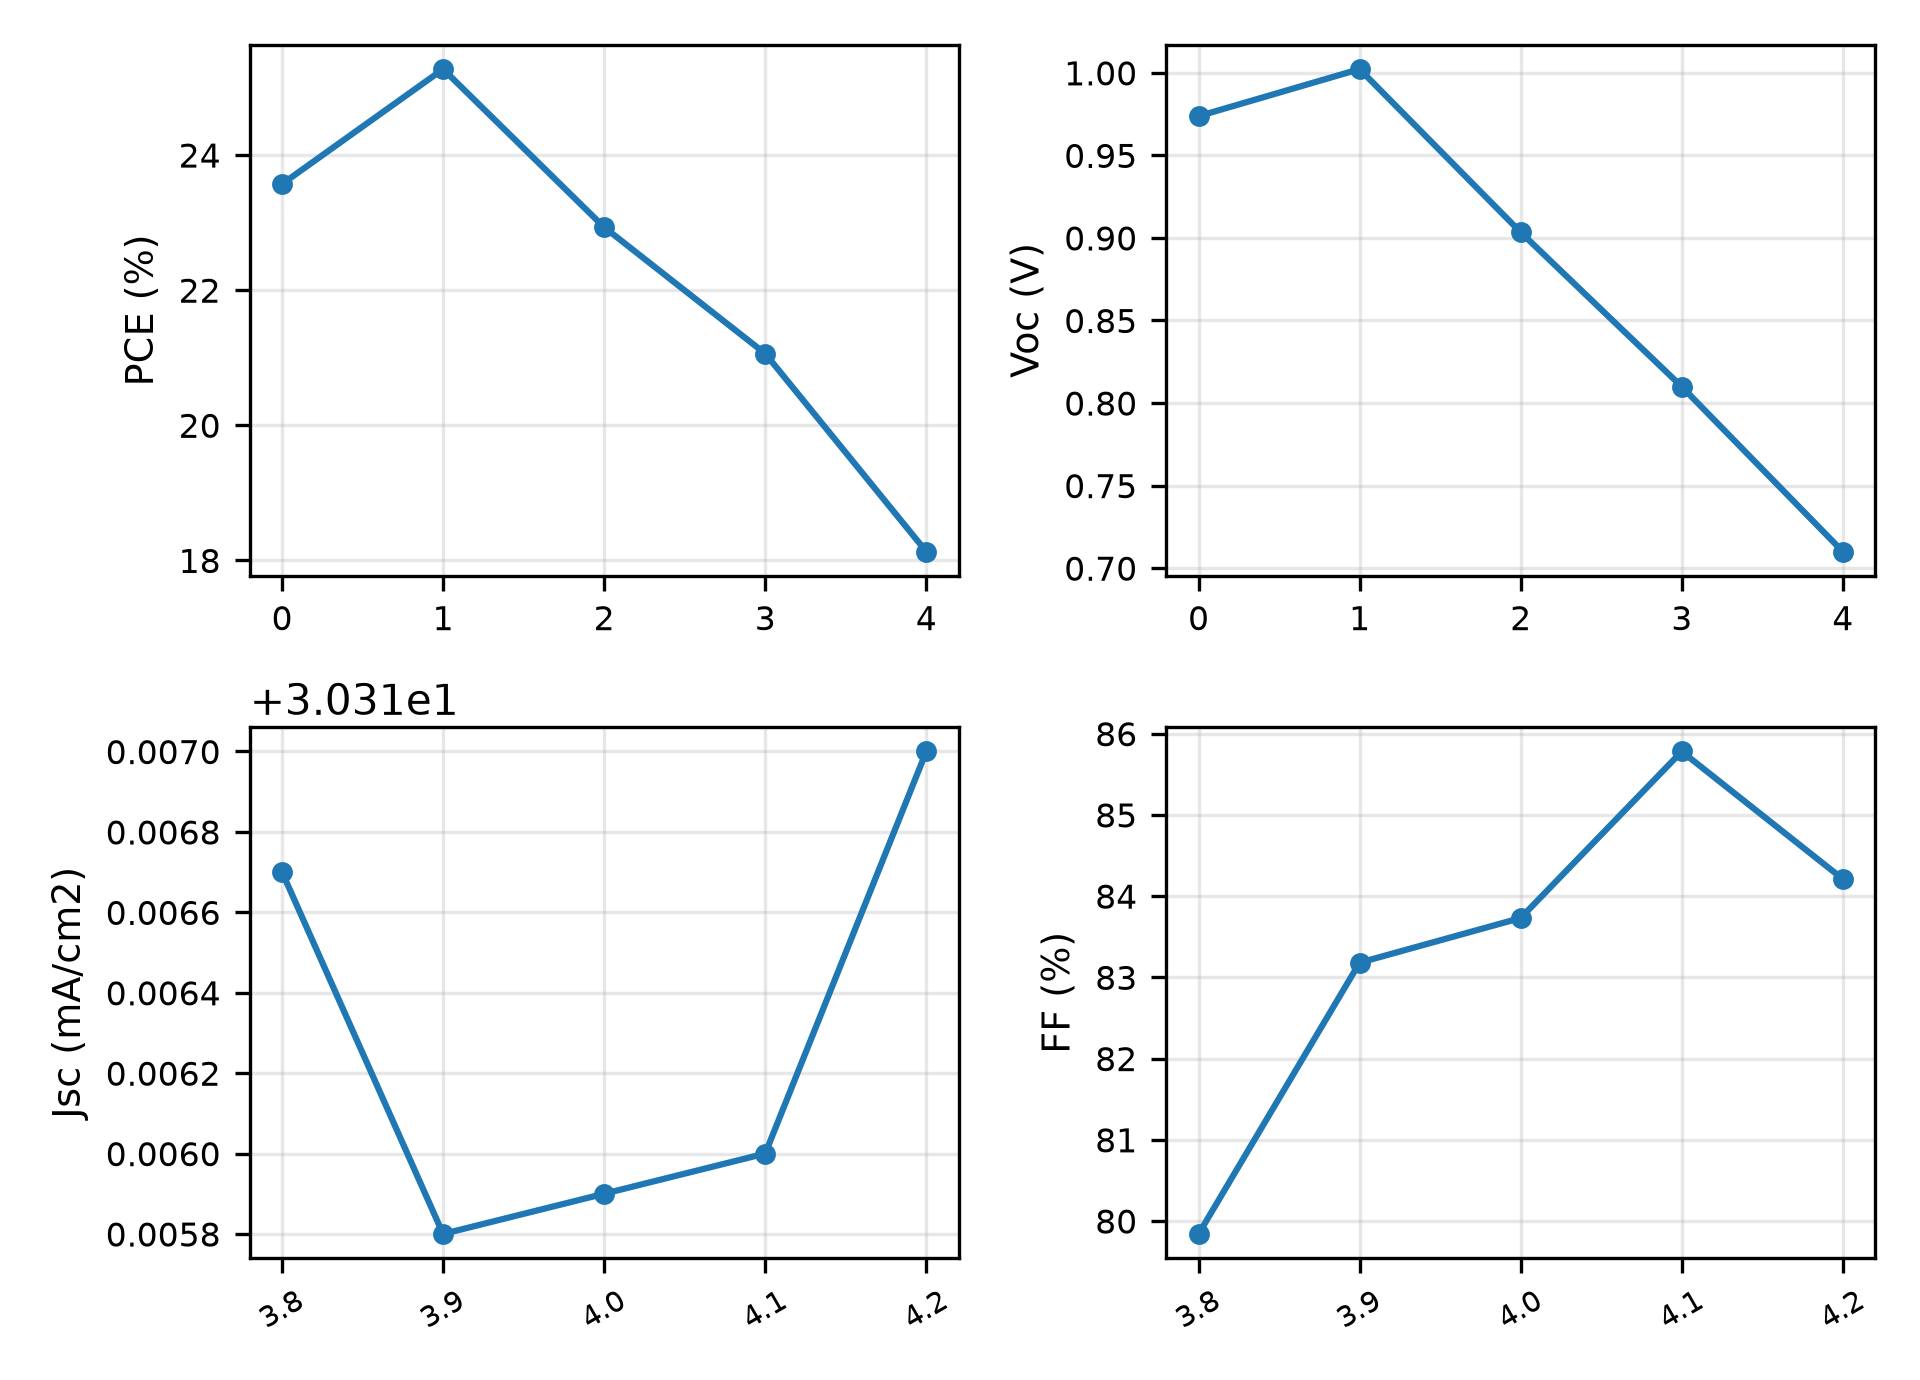
\includegraphics[width=0.85\linewidth]{figs/fig6.png}
\caption{Variation of PCE, V$_{\mathrm{OC}}$, J$_{\mathrm{SC}}$, and FF with RbGeI$_{3}$ absorber electron affinity. PCE is highest at $\chi$ = 3.9 eV due to optimal band alignment with TiO$_{2}$.}
\par\vspace{2pt}{\footnotesize\emph{Alt text: Line panels of the photovoltaic parameters against absorber dielectric constant. All four quantities are essentially flat across the range.}}\par
\end{figure}

\subsection*{Effect of TiO$_{2}$/RbGeI$_{3}$ interfacial defect density}
The TiO$_{2}$/RbGeI$_{3}$ interface is where performance is won or lost. Varying its defect density from 10$^{12}$ to 10$^{18}$ cm$^{-2}$ sends the device off a cliff: PCE drops from 25.27\% to 10.63\%, V$_{\mathrm{OC}}$ from 1.002 to 0.591 V and FF from 83.18 to 68.05\% (Figure S4), saturating past $10^{16}$ cm$^{-2}$. More states at the junction mean more carriers captured before they reach the electrodes. Best performance comes at the unphysical 10$^{12}$ cm$^{-2}$ floor, but the adopted device targets 10$^{14}$ cm$^{-2}$, a density a real film can hit and keep.


\begin{figure}[htbp]
\centering
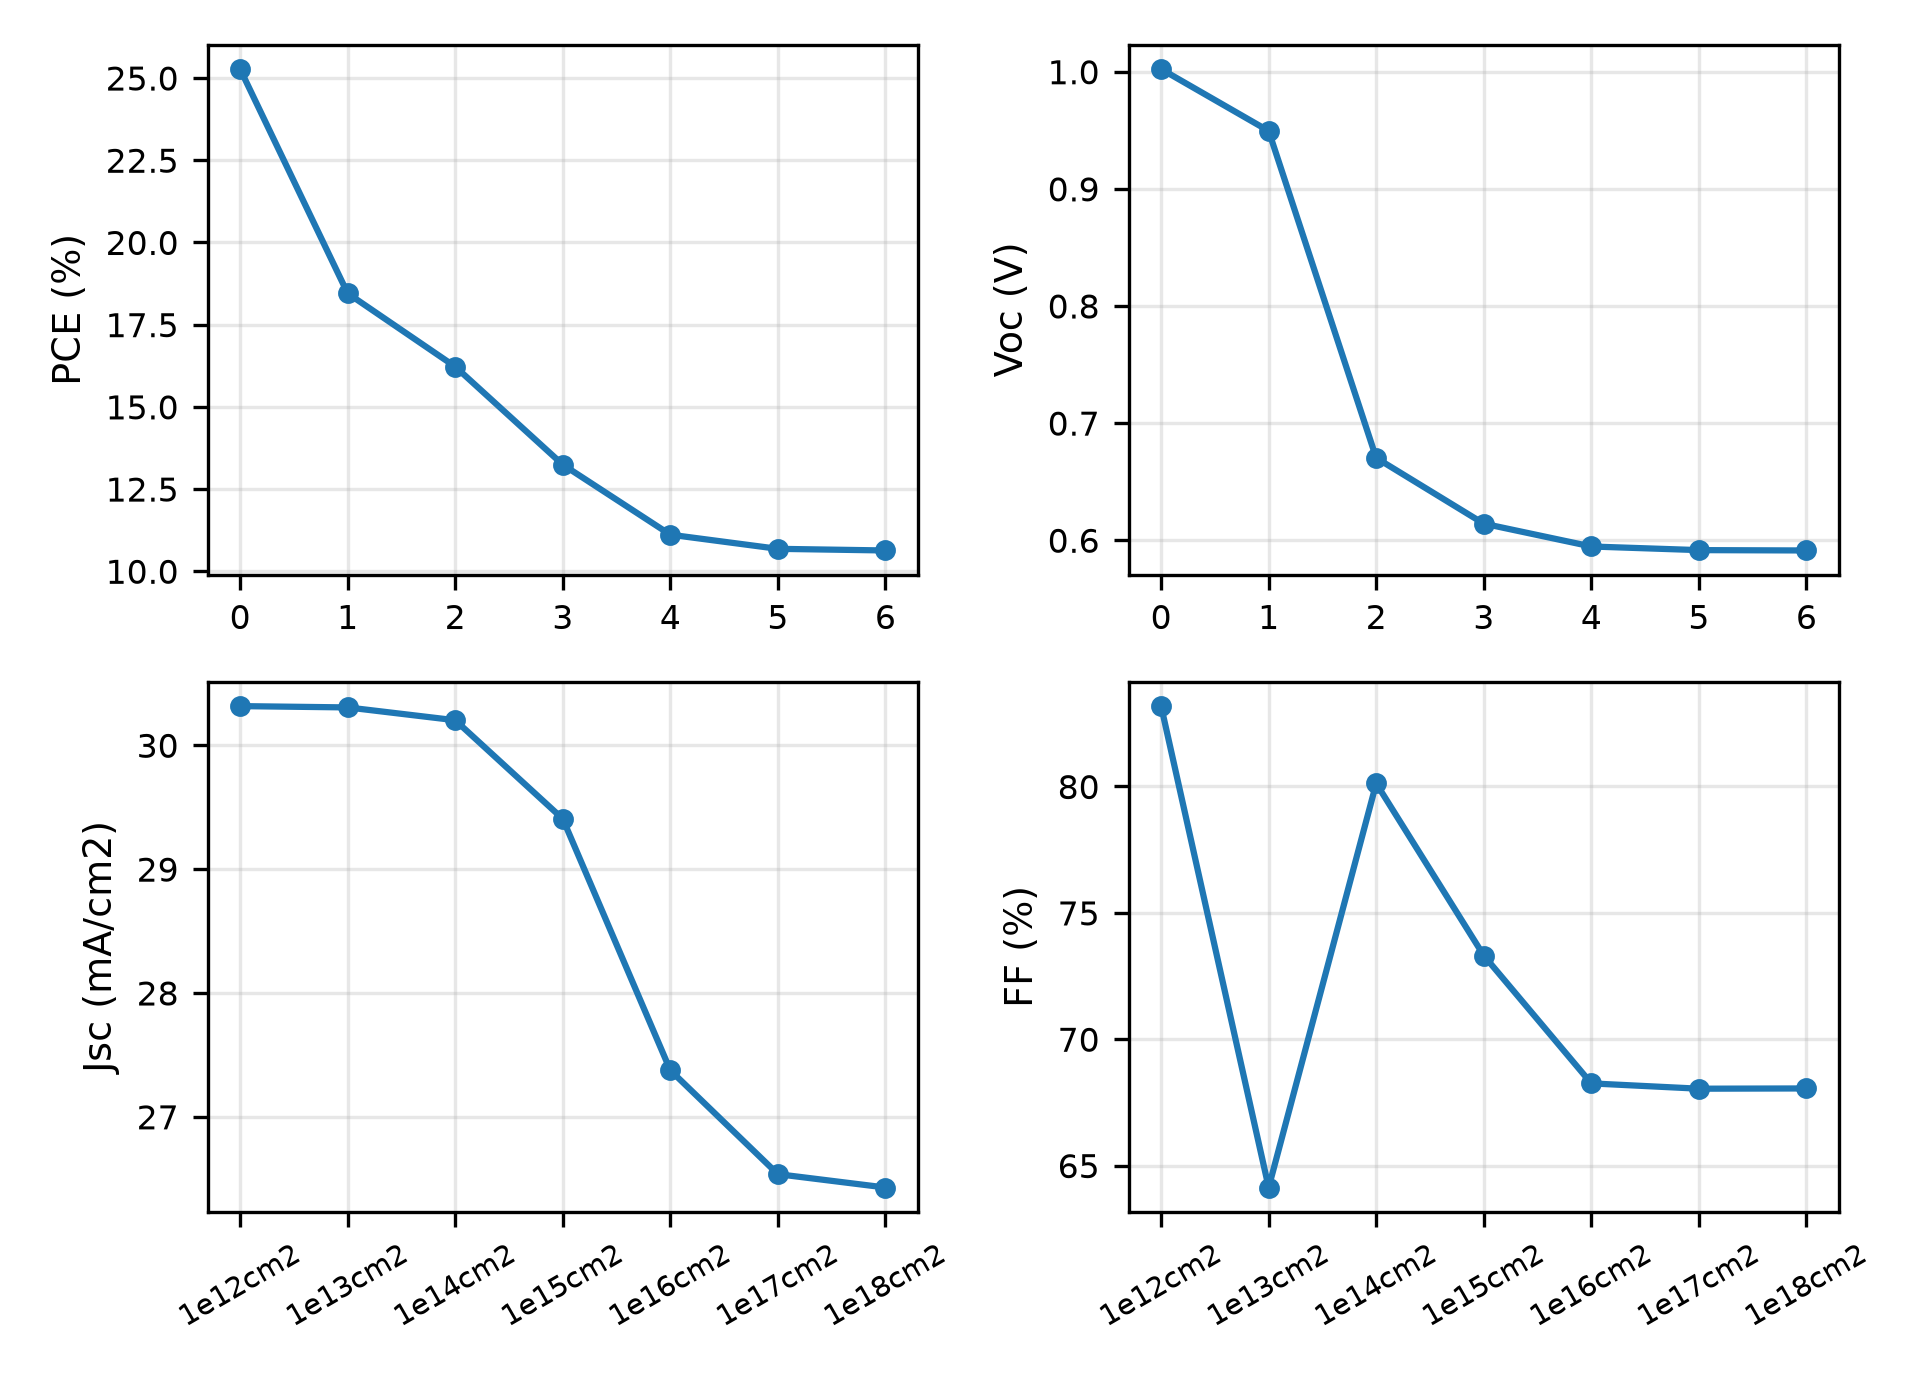
\includegraphics[width=0.85\linewidth]{figs/fig7.png}
\caption{Variation of PCE, V$_{\mathrm{OC}}$, J$_{\mathrm{SC}}$, and FF with TiO$_{2}$/RbGeI$_{3}$ interfacial defect density. Performance degrades sharply past 10$^{12}$ cm$^{-2}$ and saturates past 10$^{16}$ cm$^{-2}$; the RbGeI$_{3}$/CuI interface (Supplementary Section S1.5) is markedly more defect-tolerant.}
\par\vspace{2pt}{\footnotesize\emph{Alt text: Line panels of the photovoltaic parameters against absorber electron affinity. Performance peaks at 3.9 electronvolts, where band alignment with the electron transport layer is optimal.}}\par
\end{figure}

\subsection*{Effect of RbGeI$_{3}$/CuI interfacial defect density}
The RbGeI$_{3}$/CuI junction is far more tolerant: PCE moves only from 25.27\% to 19.85\% across the same range (Figure S5). That contrast pins the performance limit on the TiO$_{2}$/RbGeI$_{3}$ interface. The adopted device still uses 10$^{14}$ cm$^{-2}$ here for internal consistency.


\begin{figure}[htbp]
\centering
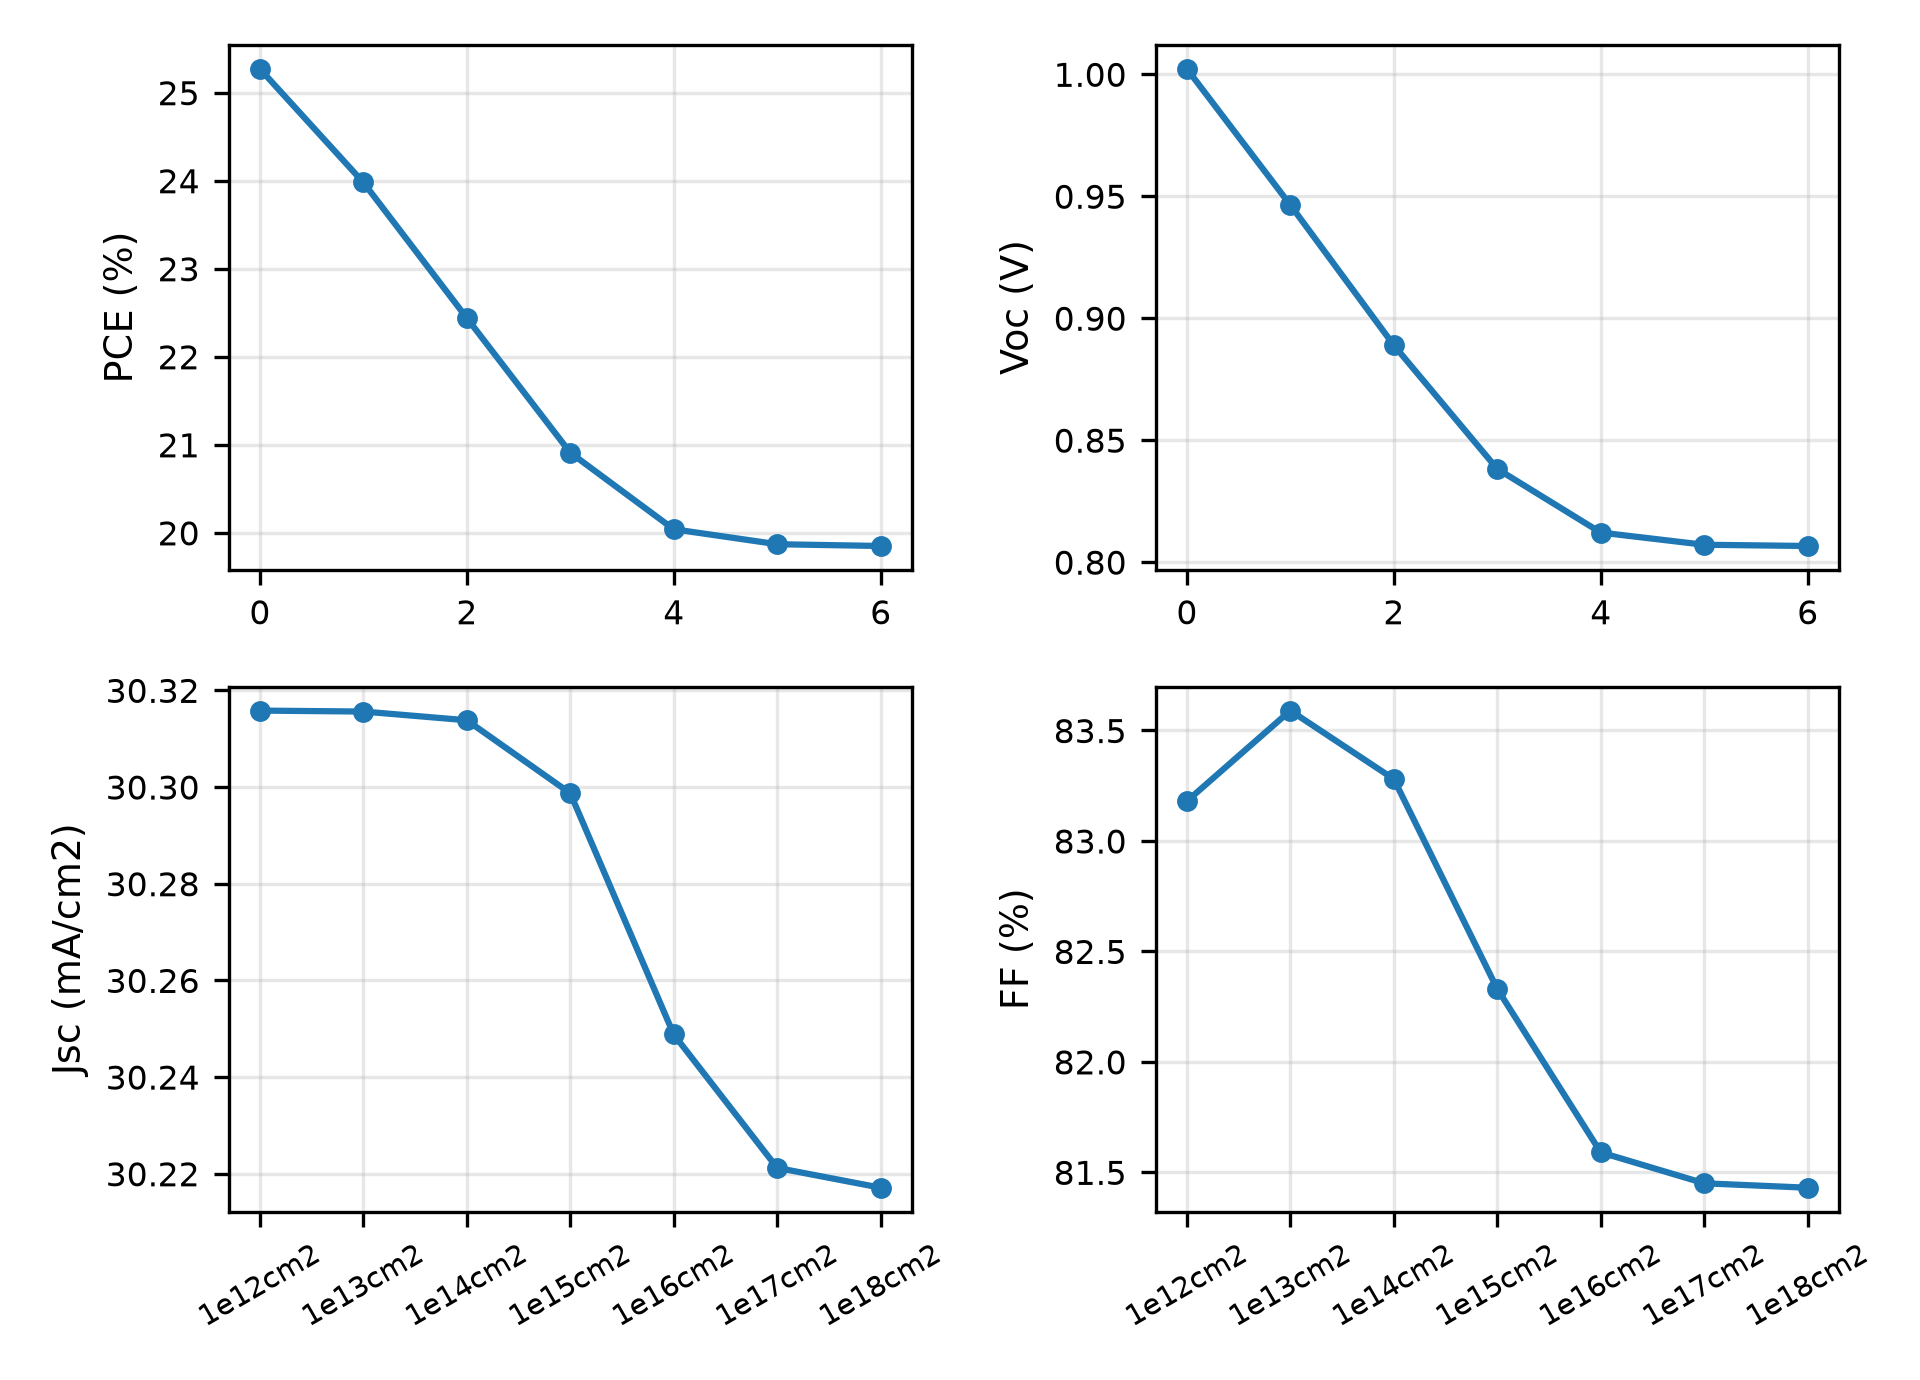
\includegraphics[width=0.85\linewidth]{figs/fig8.png}
\caption{Variation of PCE, V$_{\mathrm{OC}}$, J$_{\mathrm{SC}}$, and FF with RbGeI$_{3}$/CuI interfacial defect density. The interface is markedly more defect-tolerant than the TiO$_{2}$/RbGeI$_{3}$ interface; 10$^{14}$ cm$^{-2}$ is used here too.}
\par\vspace{2pt}{\footnotesize\emph{Alt text: Line panels of the photovoltaic parameters against the defect density at the titanium-oxide/rubidium interface. Performance degrades sharply beyond ten to the twelfth per square centimetre and saturates beyond ten to the sixteenth.}}\par
\end{figure}

\subsection*{Effect of absorber bandgap}
The bandgap picks which wavelengths the cell can use. Moving it from 1.3 to 1.7 eV, all else constant, raises V$_{\mathrm{OC}}$ from 0.966 V to 1.002 V while J$_{\mathrm{SC}}$ falls from 33.59 to 20.30 mA/cm$^{2}$ because a wider gap throws away more of the spectrum (1.4: 25.27\%; 1.5: 22.33\%; 1.6: 19.75\%; 1.7: 17.52\%).
The raw maximum sits at 1.3 eV (26.07\%), but 1.3 eV lies below the reported RbGeI$_{3}$ gap range and within 0.04 eV of the SQ optimum, so the SQ-margin gate rejects it and the absorber runs at 1.4 eV; the 1.2 eV point fails to converge. R\"uhle-tabulated SQ limits at 1.4 eV imply an ideal J$_{\mathrm{SC}}$ of 32.88 mA/cm$^{2}$ and a ceiling efficiency of 33.0\%, beside which our 30.32 mA/cm$^{2}$ and 27.06\% sit \cite{r36}. On both sides of the SQ optimum the limiting efficiency declines, steeply for wider bandgaps because fewer photons are absorbed \cite{r36,r37}: a 2.0 eV absorber would shift its absorption edge to $\lambda$c $\approx$ 620 nm and exclude most of the visible spectrum, and our sweep already shows J$_{\mathrm{SC}}$ falling to 20.30 mA/cm$^{2}$ at 1.7 eV, whereas at 1.3 eV the higher J$_{\mathrm{SC}}$ (33.59 mA/cm$^{2}$) does not offset the V$_{\mathrm{OC}}$ loss (0.966 V). The corresponding cutoff wavelength is $\lambda$c = 1240 / 1.4 $\approx$ 886 nm, consistent with the square-root-law absorption edge used in the generation profile of the main text. A targeted re-simulation varying only the absorption-grading endpoints (graded 885.7--1033.3 nm versus flat 885.7--885.7 nm, all else fixed) changes J$_{\mathrm{SC}}$ by 0.00 mA/cm$^{2}$, and the consolidated J$_{\mathrm{SC}}$ of 30.32 mA/cm$^{2}$ lies below the SQ limit of $\approx$33 mA/cm$^{2}$ at 1.4 eV, so the headline result is admissible with uniform square-root-law absorption at the electrical bandgap; the 27.06\% device is therefore reported as an ideal-coupling upper bound, with a quantified realistic window given in Sections V.G and VII.A of the main text.


\begin{figure}[htbp]
\centering
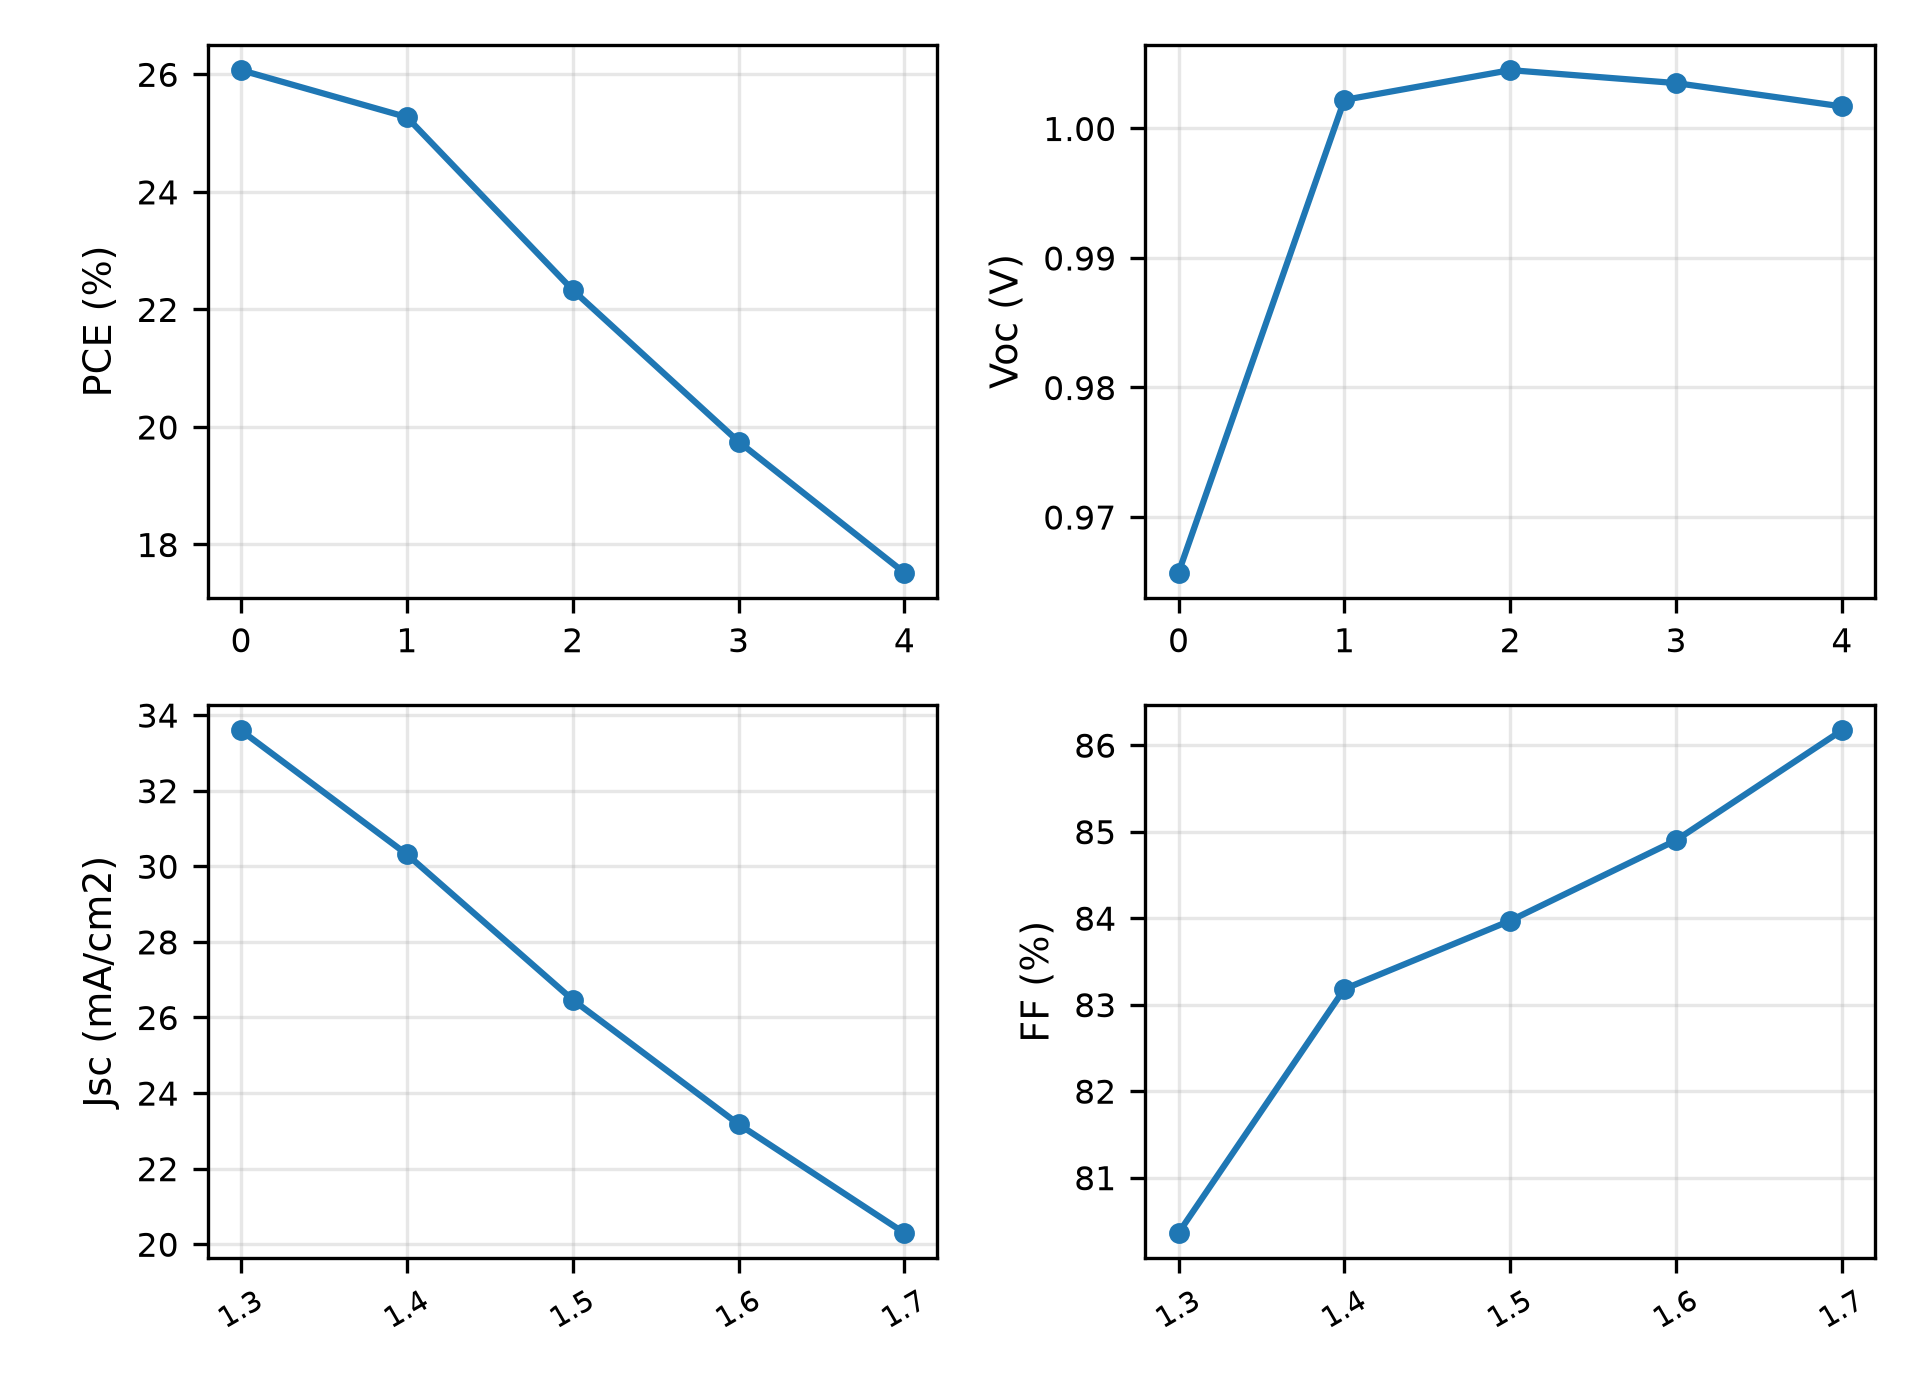
\includegraphics[width=0.85\linewidth]{figs/fig9.png}
\caption{Variation of PCE, V$_{\mathrm{OC}}$, J$_{\mathrm{SC}}$, and FF with RbGeI$_{3}$ absorber bandgap. The raw peak at 1.3 eV is rejected by the SQ-margin gate; 1.4 eV is adopted.}
\par\vspace{2pt}{\footnotesize\emph{Alt text: Line panels of the photovoltaic parameters against the defect density at the rubidium/copper-iodide interface. The interface is markedly more defect-tolerant; ten to the fourteenth per square centimetre is used.}}\par
\end{figure}

\subsection*{Effect of TiO$_{2}$ ETL thickness}
Thickness of the TiO$_{2}$ ETL cuts across electron extraction, transport, and optical transmission at once. Sweeping it from 10 to 90 nm, all else fixed, gives the best PCE at the thinnest layer: 29.09\% at 10 nm, a sharp local low of 21.39\% at 40 nm (FF collapses to 70.24\%, reproduced on re-run --- a genuine solver anomaly disclosed, not hidden), and a partial recovery to 25.33\% at 90 nm (20 nm: 28.19\%, cost of a pinhole-safe choice $\approx$0.9 pp). Planar SCAPS studies stick to thin ($\leq$50 nm) ETLs for the same reason we do: thicker ones add series resistance and soak up photons.


\begin{figure}[htbp]
\centering
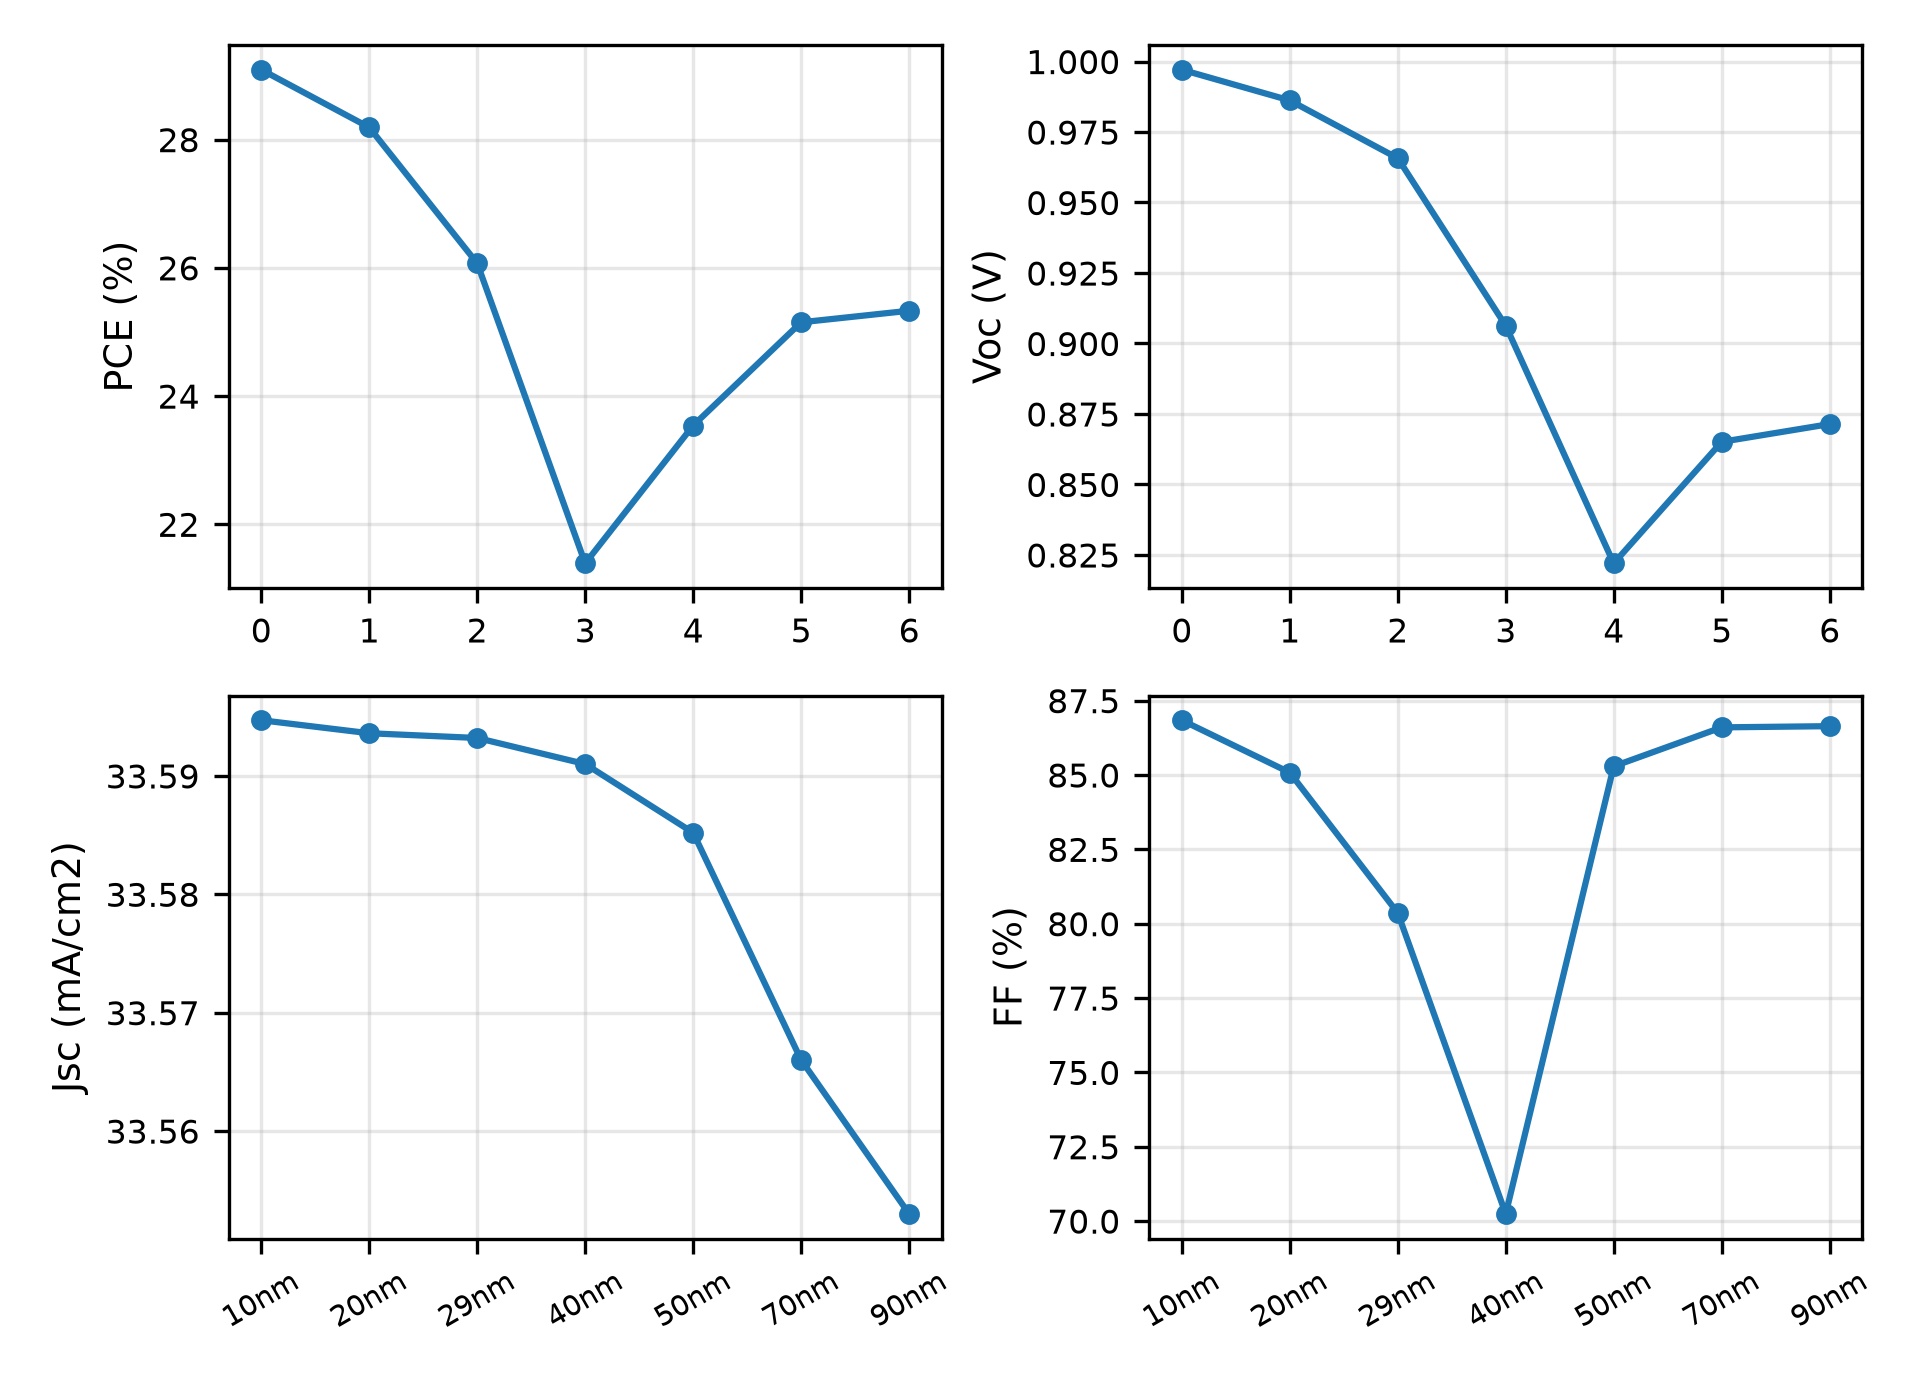
\includegraphics[width=0.85\linewidth]{figs/fig10.png}
\caption{Variation of PCE, V$_{\mathrm{OC}}$, J$_{\mathrm{SC}}$, and FF with TiO$_{2}$ ETL thickness. PCE is highest at the thinnest ETL (10 nm), reflecting the shorter electron transport path.}
\par\vspace{2pt}{\footnotesize\emph{Alt text: Line panels of the photovoltaic parameters against absorber bandgap. The raw maximum at 1.3 electronvolts is rejected by the margin gate and 1.4 is adopted.}}\par
\end{figure}

\subsection*{Effect of CuI HTL thickness}
CuI thickness, swept from 0.05 to 1.9 $\mu$m, leaves PCE bit-identical at 29.09\% at every point; V$_{\mathrm{OC}}$, J$_{\mathrm{SC}}$, and FF are constant to four figures. That flatness lets us pick 100 nm purely to minimize material use. It sits at the low end of the 0.1--1.0 $\mu$m range comparable studies explored, which also reported a weak dependence.


\begin{figure}[htbp]
\centering
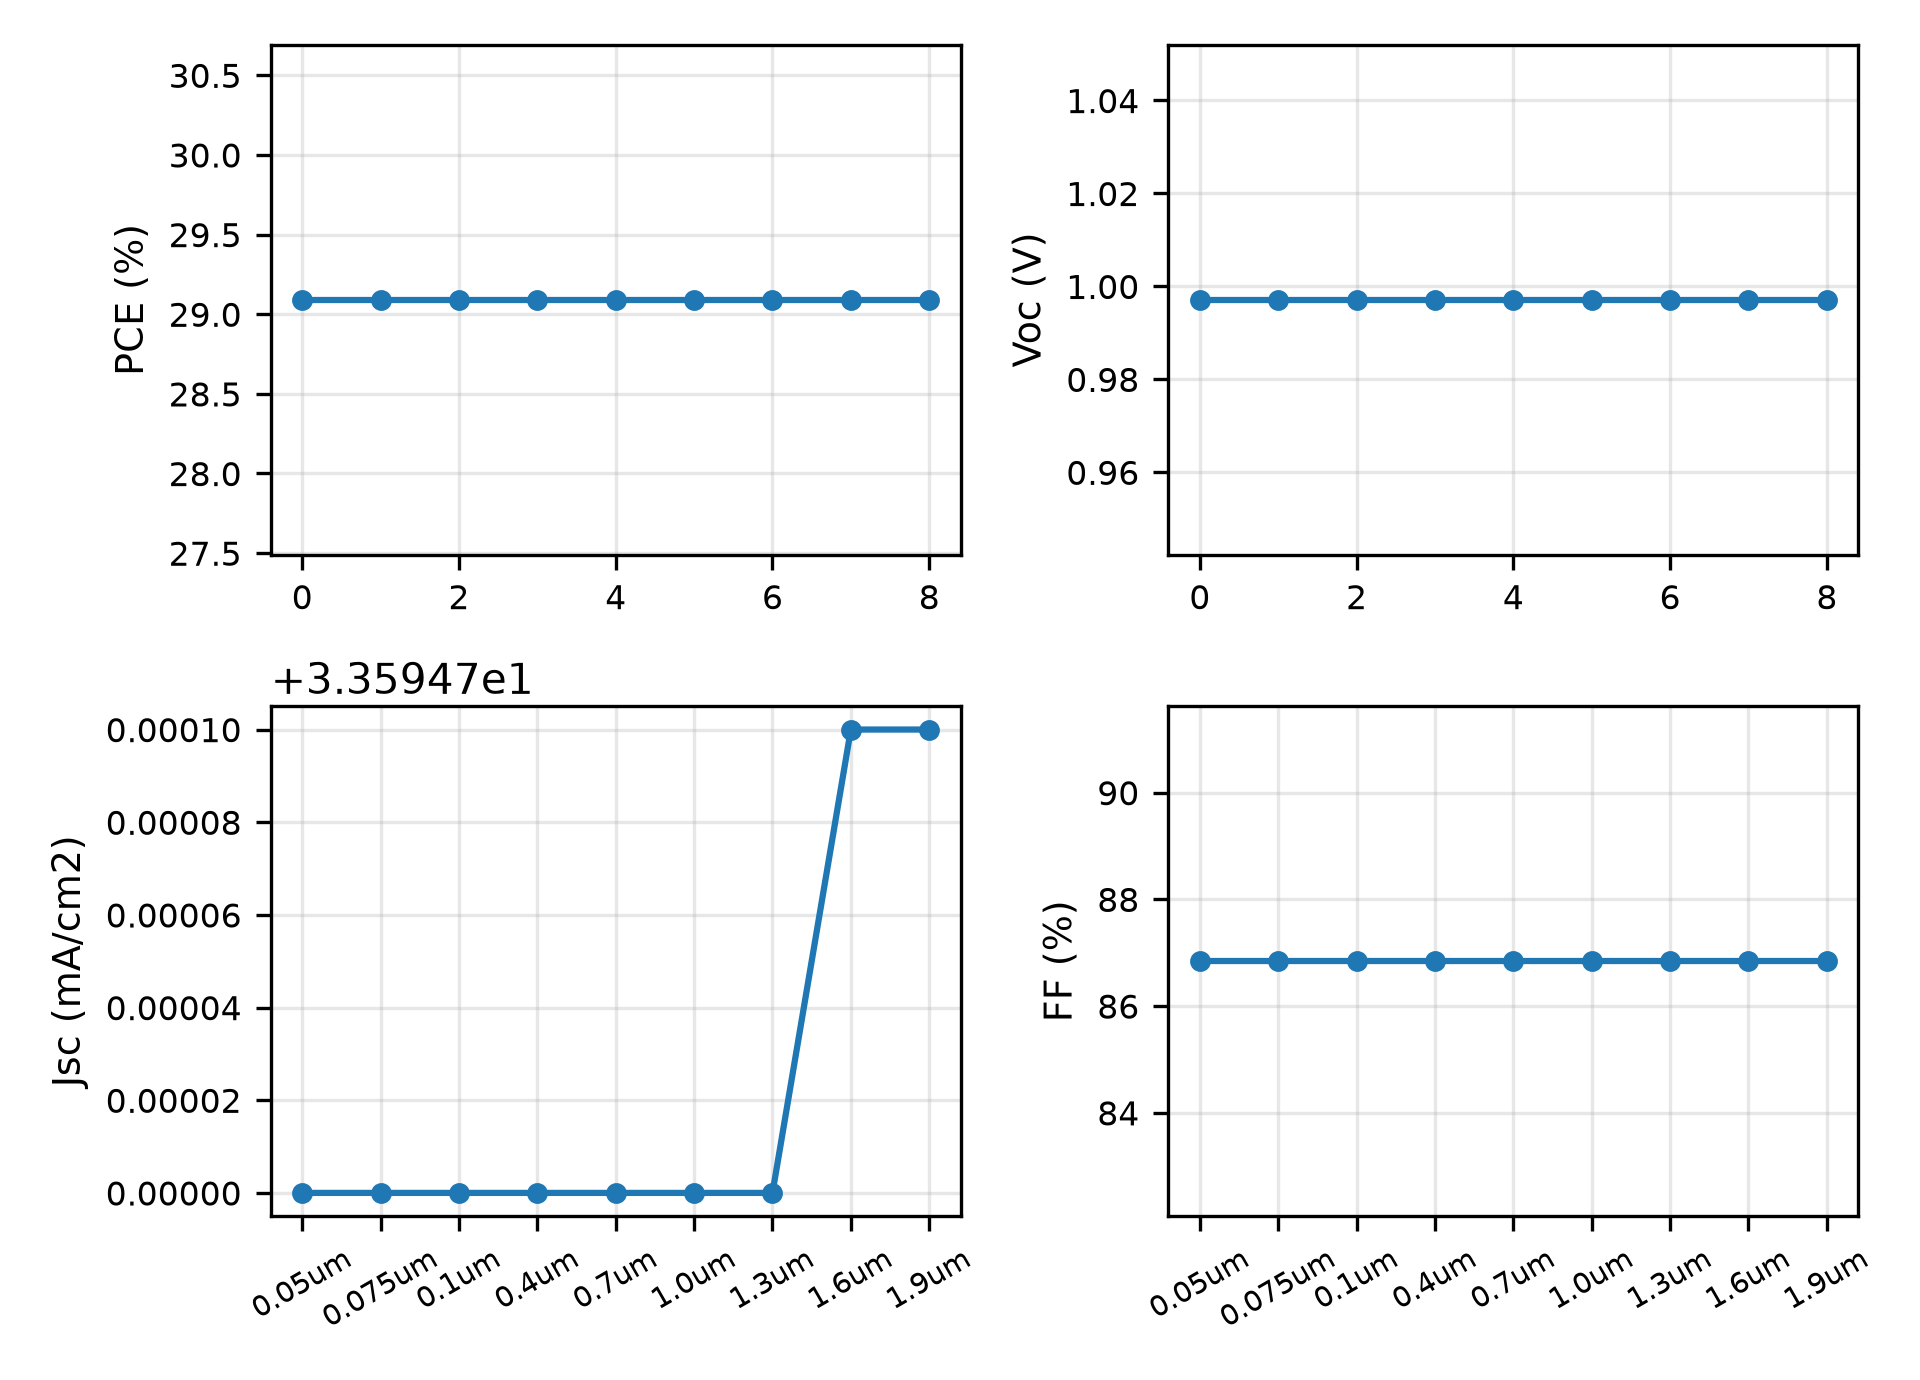
\includegraphics[width=0.85\linewidth]{figs/fig11.png}
\caption{Variation of PCE, V$_{\mathrm{OC}}$, J$_{\mathrm{SC}}$, and FF with CuI HTL thickness. The performance is essentially independent of HTL thickness; 100 nm minimizes material usage.}
\par\vspace{2pt}{\footnotesize\emph{Alt text: Line panels of the photovoltaic parameters against electron-transport-layer thickness. Performance peaks at the thinnest ten-nanometre layer, reflecting the shorter electron path.}}\par
\end{figure}

\subsection*{Effect of conduction-band effective density of states N$_{\mathrm{C}}$}
Raising N$_{\mathrm{C}}$ from 1$\times$10$^{18}$ to 1$\times$10$^{20}$ cm$^{-3}$ pushes PCE monotonically down from 30.01\% to 27.60\%; V$_{\mathrm{OC}}$ carries the loss (1.037 to 0.950 V) while J$_{\mathrm{SC}}$ sits bit-flat at 33.59 mA/cm$^{2}$. A lower N$_{\mathrm{C}}$ means a lower intrinsic carrier density and therefore a higher V$_{\mathrm{OC}}$, so the bottom of the literature-floor sweep, 1$\times$10$^{18}$ cm$^{-3}$, goes into the adopted device; probing one decade below the floor gains only 0.13 pp, so the floor pin stands.


\begin{figure}[htbp]
\centering
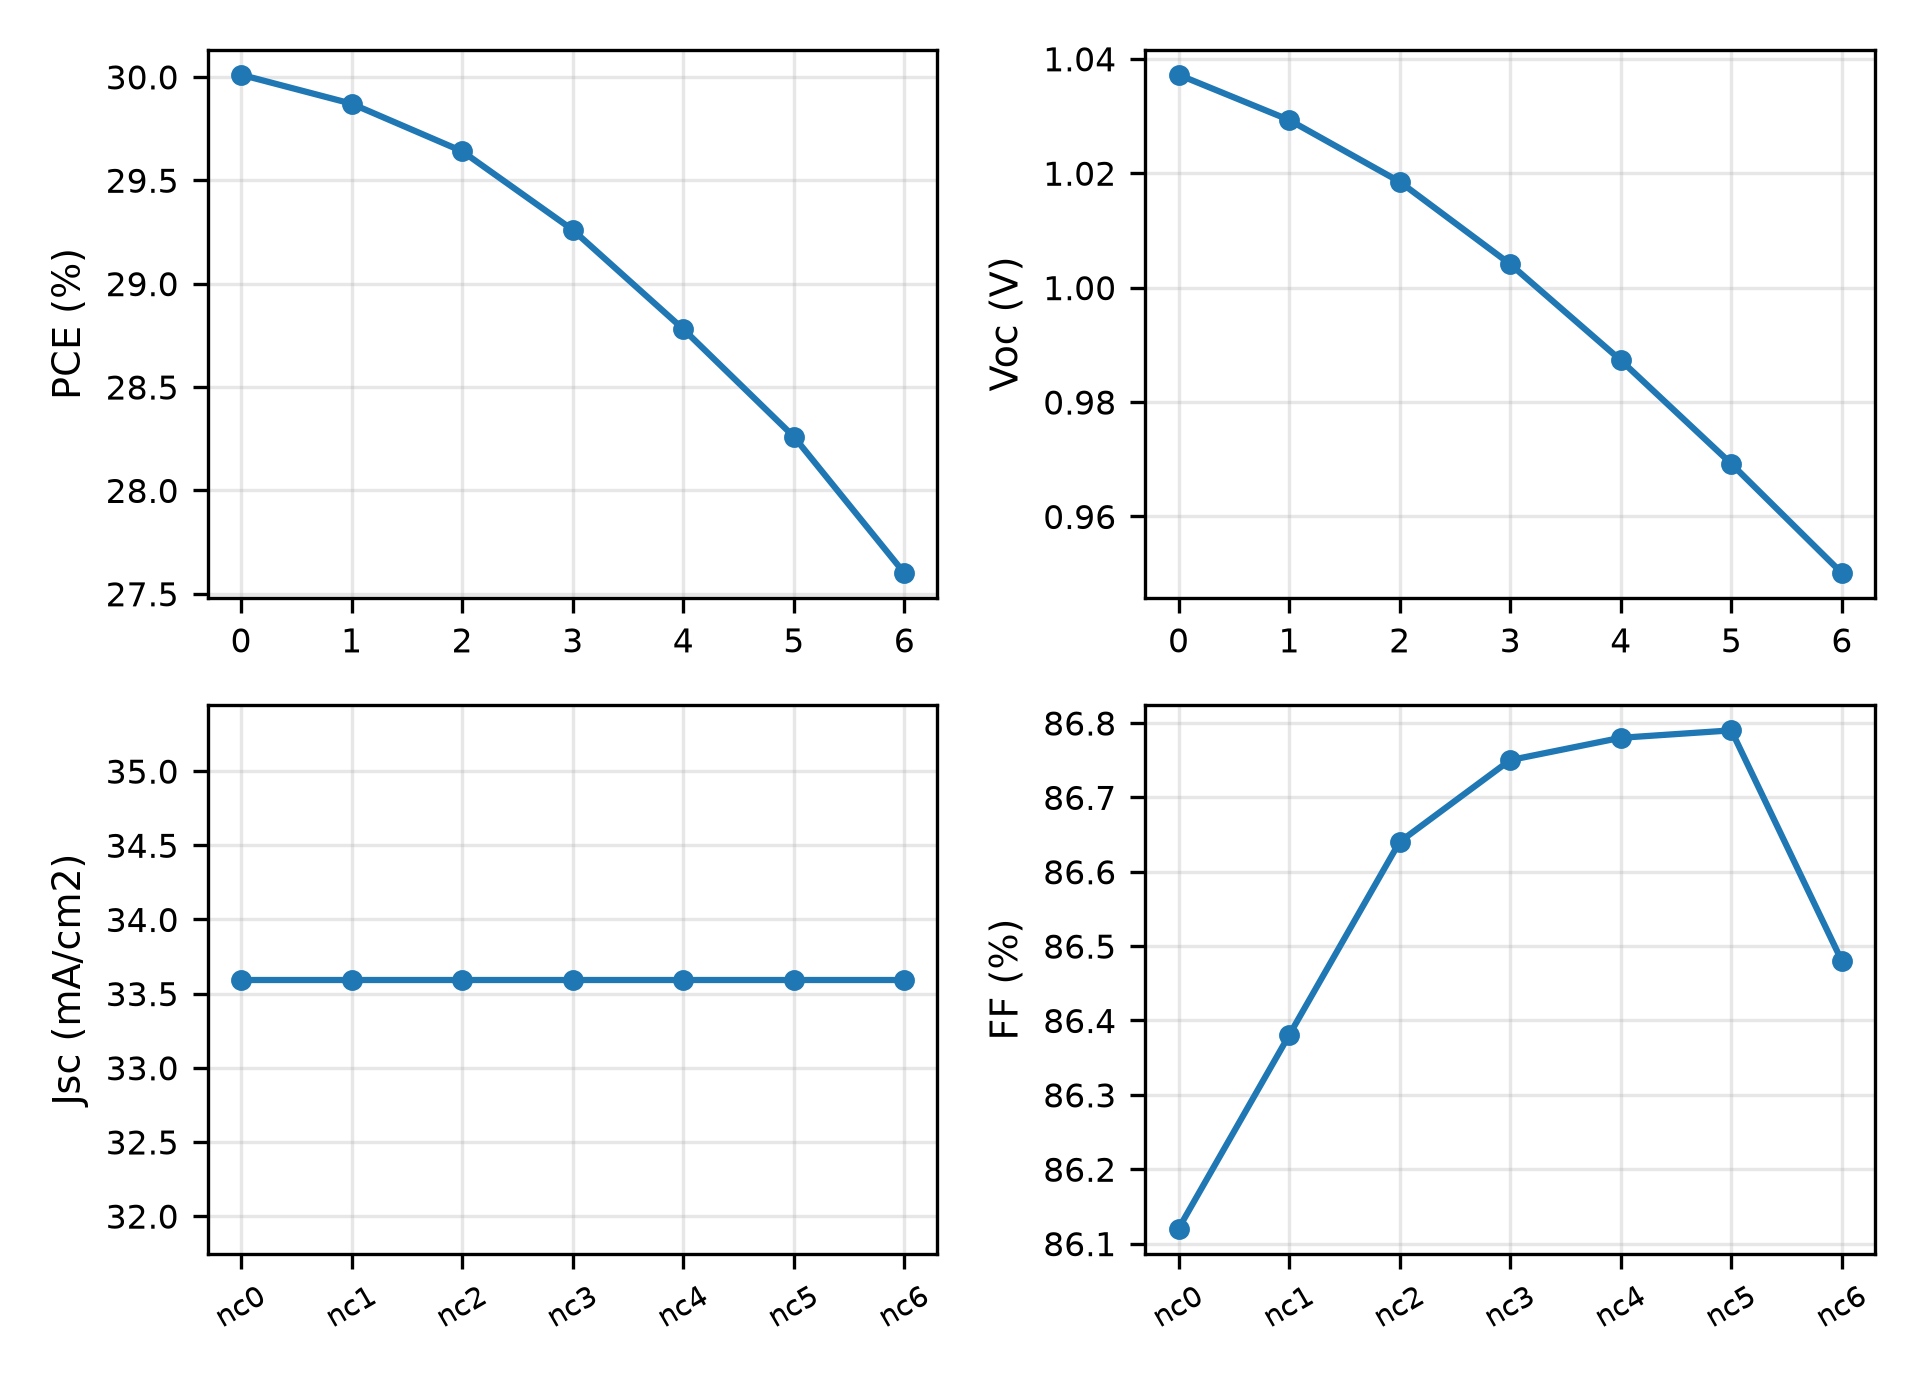
\includegraphics[width=0.85\linewidth]{figs/fig12.png}
\caption{Variation of PCE, V$_{\mathrm{OC}}$, J$_{\mathrm{SC}}$, and FF with conduction-band effective density of states N$_{\mathrm{C}}$. Lower N$_{\mathrm{C}}$ is preferred; the adopted literature-floor value is 10$^{18}$ cm$^{-3}$.}
\par\vspace{2pt}{\footnotesize\emph{Alt text: Line panels of the photovoltaic parameters against hole-transport-layer thickness. Performance is essentially flat, so 100 nanometres minimizes material use.}}\par
\end{figure}

\subsection*{Effect of valence-band effective density of states N$_{\mathrm{V}}$}
N$_{\mathrm{V}}$ behaves like N$_{\mathrm{C}}$ but hits harder. Across 1$\times$10$^{18}$ to 1$\times$10$^{20}$ cm$^{-3}$, PCE drops from 31.57\% to 29.05\% as V$_{\mathrm{OC}}$ slides from 1.074 to 1.010 V with J$_{\mathrm{SC}}$ flat at $\approx$33.59 mA/cm$^{2}$. The smallest value wins again: N$_{\mathrm{V}}$ = 1$\times$10$^{18}$ cm$^{-3}$ is carried into the adopted set; sub-floor probing gains only 0.04 pp.


\begin{figure}[htbp]
\centering
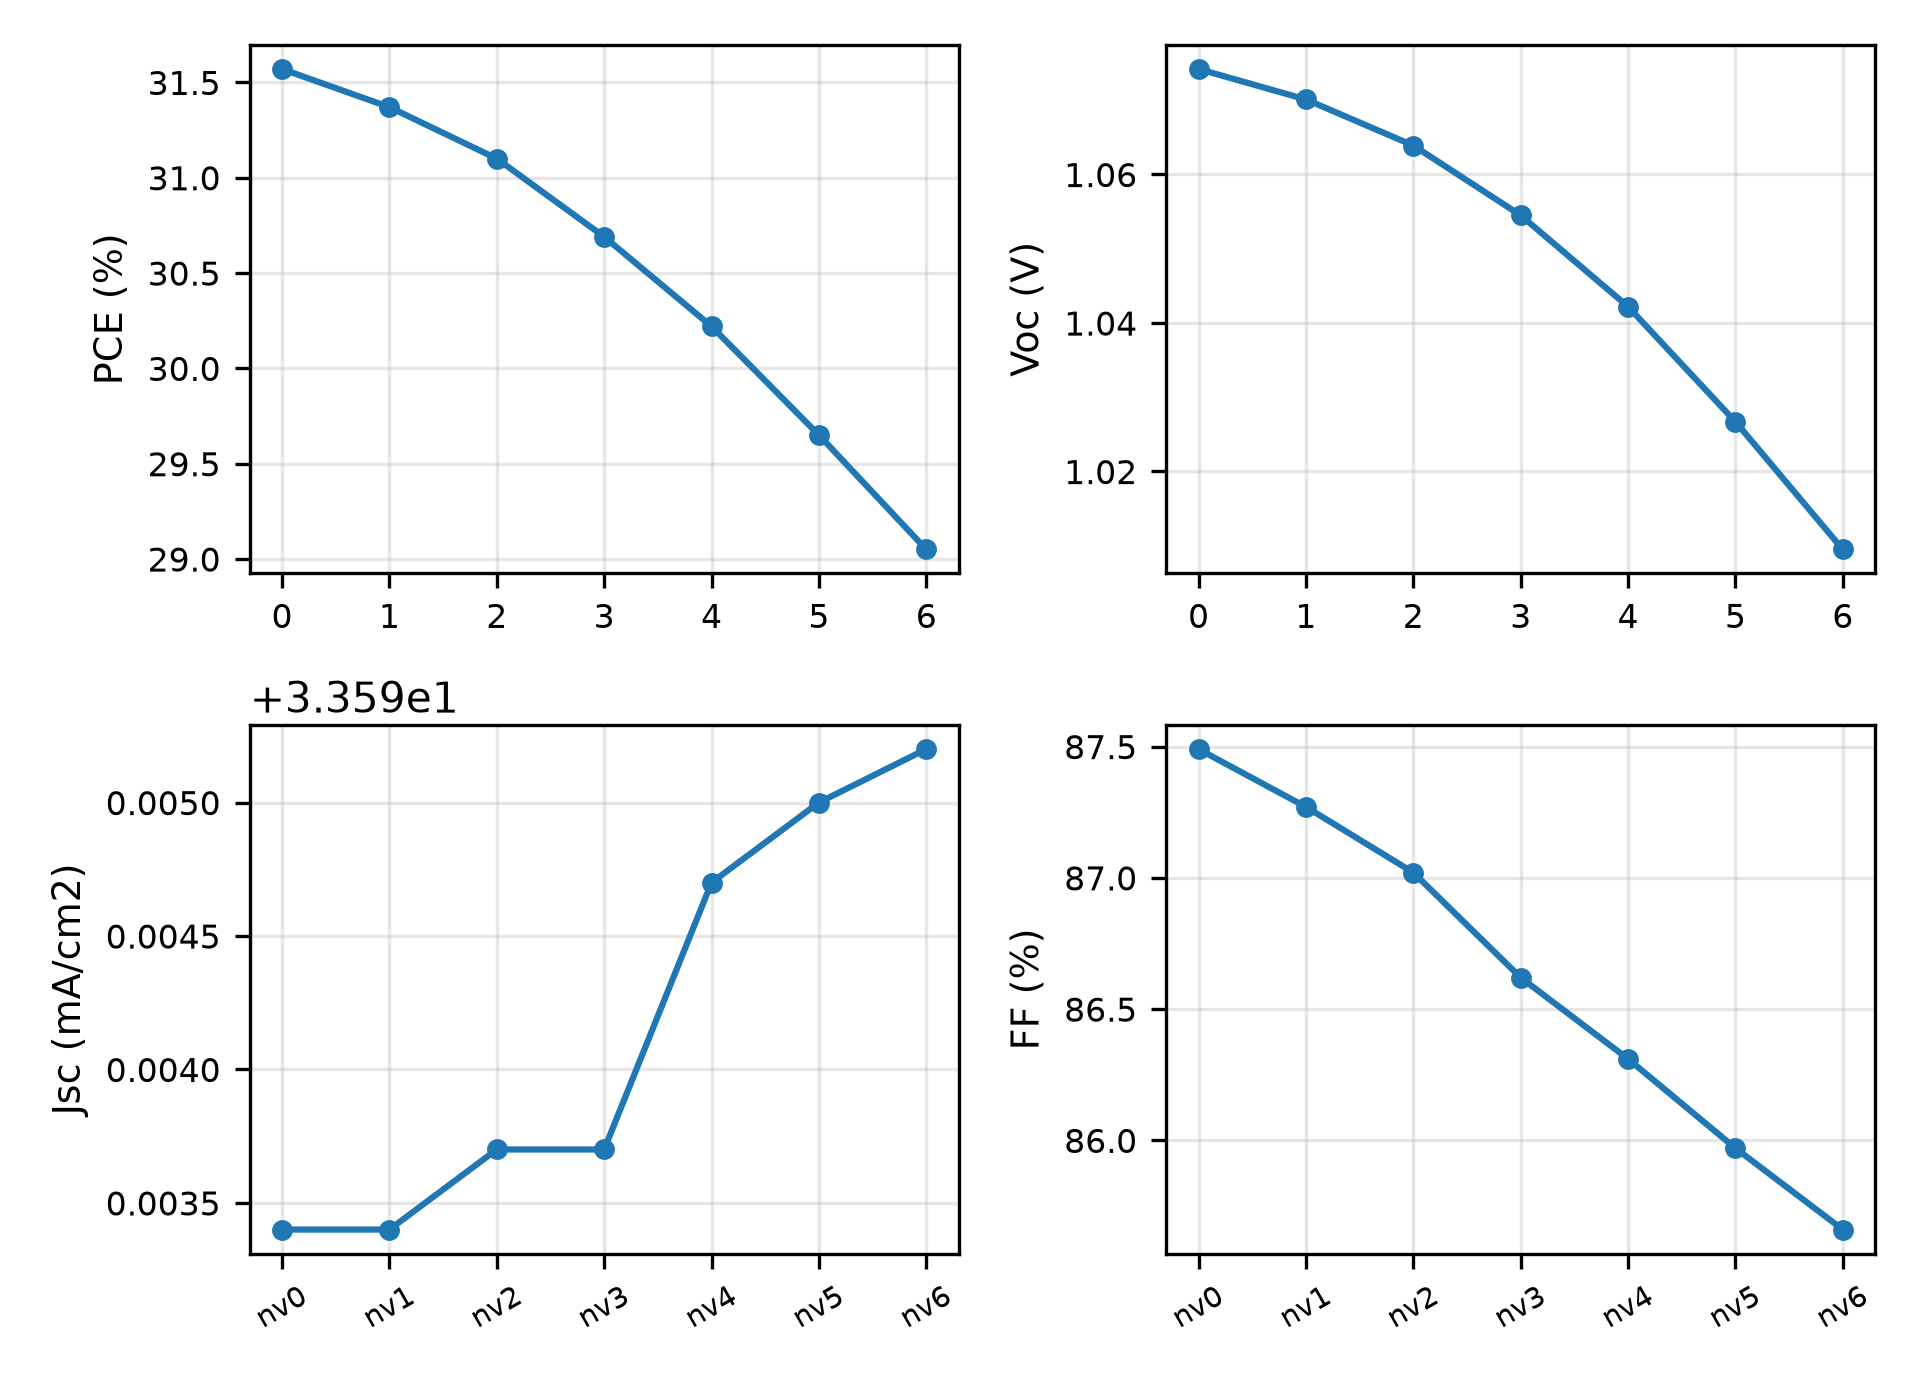
\includegraphics[width=0.85\linewidth]{figs/fig13.png}
\caption{Variation of PCE, V$_{\mathrm{OC}}$, J$_{\mathrm{SC}}$, and FF with valence-band effective density of states N$_{\mathrm{V}}$. The effect is more pronounced than for N$_{\mathrm{C}}$; the adopted literature-floor value is 10$^{18}$ cm$^{-3}$.}
\par\vspace{2pt}{\footnotesize\emph{Alt text: Line panels of the photovoltaic parameters against conduction-band density of states. Lower values are preferred and the literature-floor value of ten to the eighteenth is adopted.}}\par
\end{figure}

\subsection*{D2 like-for-like pipeline (TiO$_{2}$/NiO stack)}
D2 ran the identical eleven-step chain on its own NiO deck (same grids, raw-maximum carry-forward, same triple-gate assembly). Step maxima (carried): thickness 0.8 $\mu$m (21.30\%); bulk $N_{t}$ $10^{12}$ cm$^{-3}$ (26.46\%); $\epsilon_{r}$ 23.1 (26.46\%); $\chi$ 3.9 (26.46\%, bracketed by non-convergent 3.7/4.2); TiO$_{2}$-side $N_{t}$ $10^{12}$ cm$^{-2}$ (26.46\%); NiO-side $N_{t}$ $10^{12}$ cm$^{-2}$ (26.46\%, degrading gracefully to 22.81\% at $10^{18}$); $E_{g}$ 1.4 eV (26.46\%); ETL 10 nm (30.16\%, with the 40 nm anomaly reproduced at 22.44\%); HTL flat at 30.16\%; $N_{C}$ $10^{18}$ cm$^{-3}$ (30.38\%); $N_{V}$ $10^{18}$ cm$^{-3}$ (32.87\%). Gate-adopted D2: 28.16\% (1.1116 V, 30.3154 mA/cm$^{2}$, 83.57\%). Archives: \texttt{r8\_D2\_s\_*.json}, chain record \texttt{r8\_D2\_chain.json}, deck \texttt{r8\_D2\_H1\_adopted.def}, J--V \texttt{r8\_D2\_H1\_JV.json}.

\section*{S2.\ Illumination and dark characteristics}
\subsection*{Illumination dependence}
The optimized cell was also driven under 0.1 to 1.5 suns (Figure S11). J$_{\mathrm{SC}}$ tracks intensity almost linearly, the natural consequence of carrier generation scaling with photon flux, while V$_{\mathrm{OC}}$ rises logarithmically. The slope of that logarithmic rise gives an ideality factor n $\approx$ 1.17, so deep-defect Shockley-Read-Hall recombination is not dominant under operating conditions, and the cell stays efficient across the entire range. Re-simulation on the rebased deck (0.1--1.5 suns, archived \texttt{r8\_darkillum.json}) gives J$_{\mathrm{SC}}$ = 3.03/9.09/15.16/24.25/30.32/45.47 mA/cm$^{2}$ (perfect linearity) and n = 1.19 from the V$_{\mathrm{OC}}$--ln(I) slope over 0.3--1.5 suns, confirming the reported n $\approx$ 1.2.


\begin{figure}[htbp]
\centering
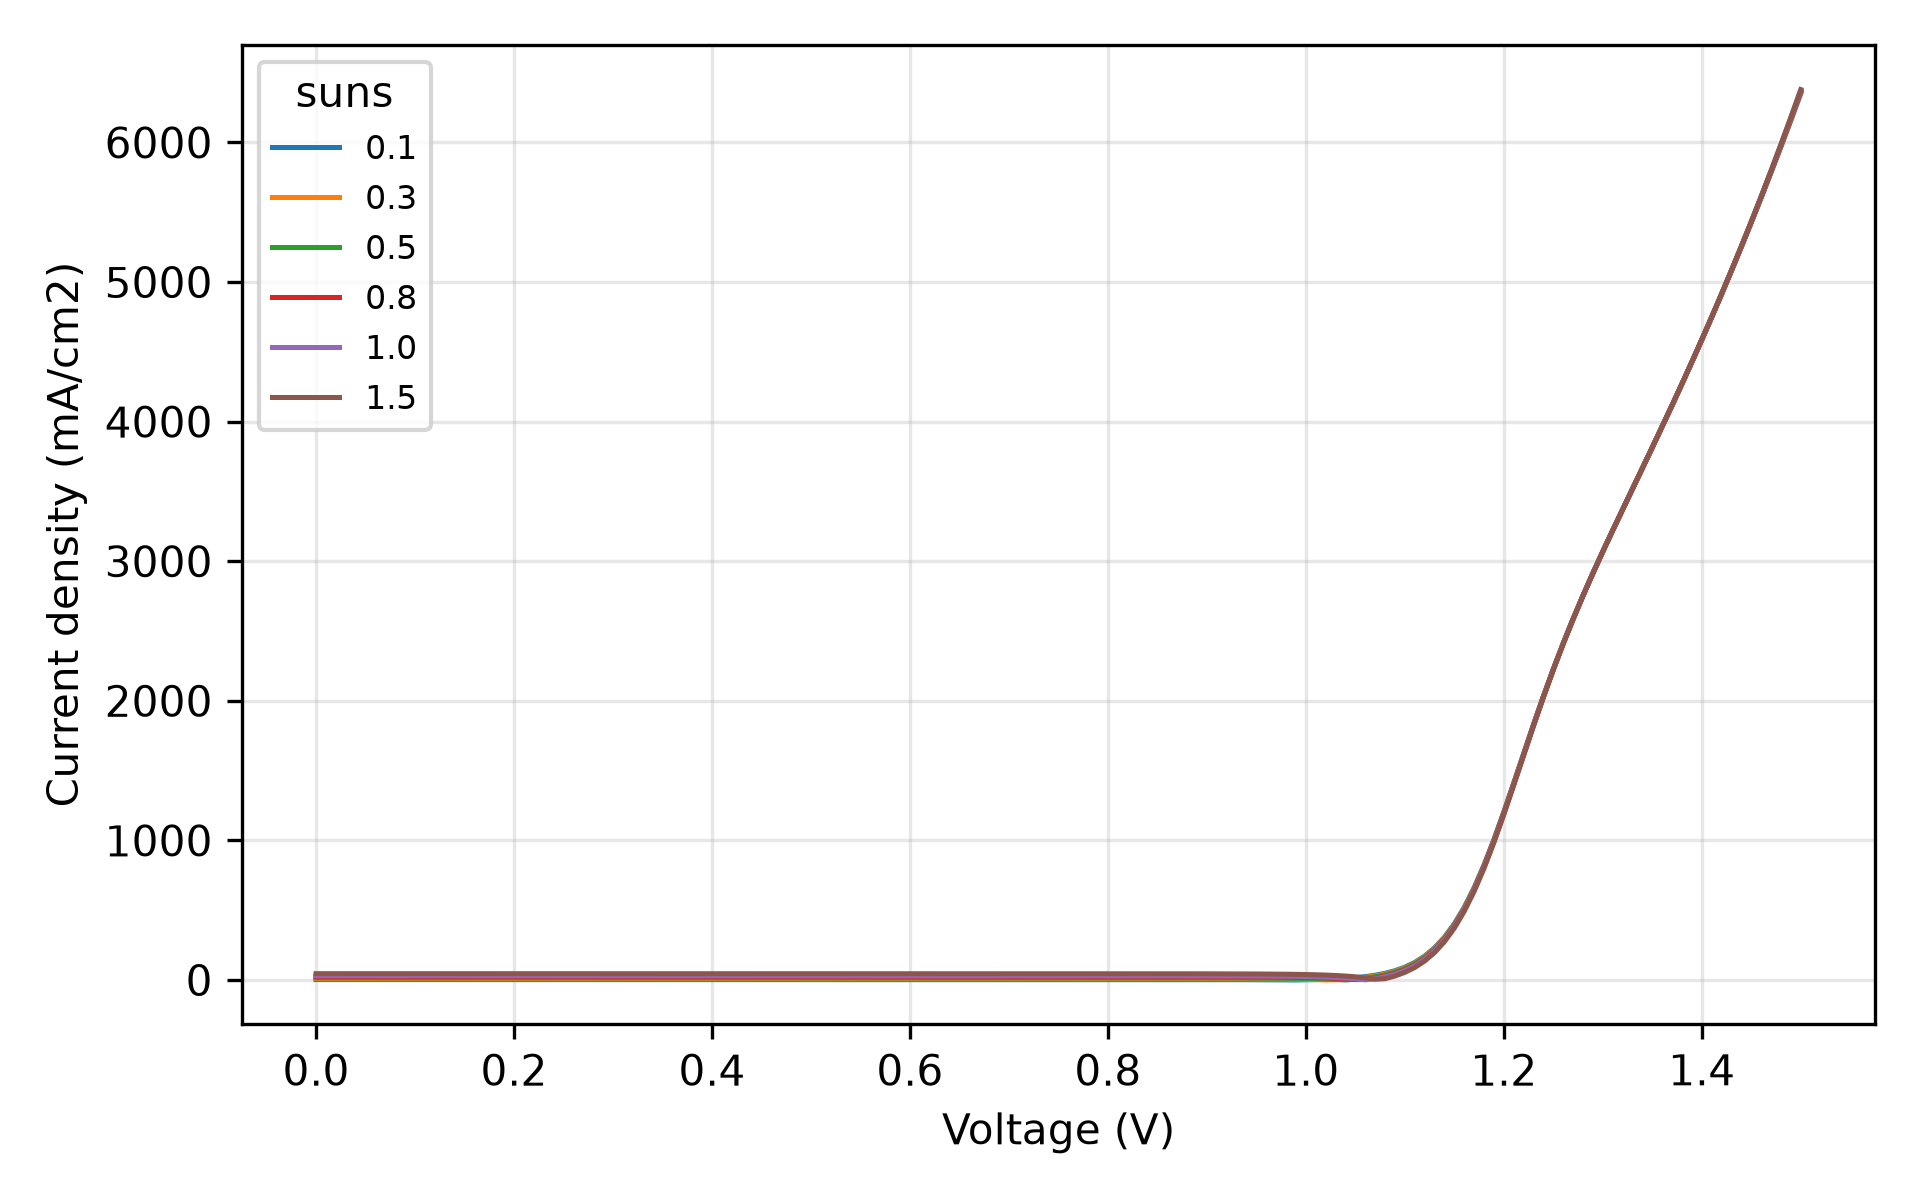
\includegraphics[width=0.85\linewidth]{figs/fig18.png}
\caption{Variation of photovoltaic parameters of the optimized device with illumination intensity from 0.1 to 1.5 suns.}
\par\vspace{2pt}{\footnotesize\emph{Alt text: Four-panel plot of the optimized device versus illumination intensity from 0.1 to 1.5 suns. Current rises almost linearly with light level while voltage rises logarithmically.}}\par
\end{figure}

\subsection*{Dark J--V characteristics}
Under dark bias (Figure S12, archived \texttt{r8\_dark\_JV.json}) the cell rectifies hard: forward current at +1 V exceeds reverse current at $-$0.5 V by a factor of 1.7$\times$10$^{10}$, and leakage stays under 10$^{-10}$ A/cm$^{2}$ across the whole reverse window. The low-bias exponential forward region (0.2--0.6 V, $r=0.9986$) fits to an ideality factor n $\approx$ 1.2 and J0 $\approx$ 6$\times$10$^{-11}$ A/cm$^{2}$; higher-bias windows bend upward from series/high-injection effects and are not used. Together these numbers describe high-quality bulk and interfaces with no measurable shunts.


\begin{figure}[htbp]
\centering
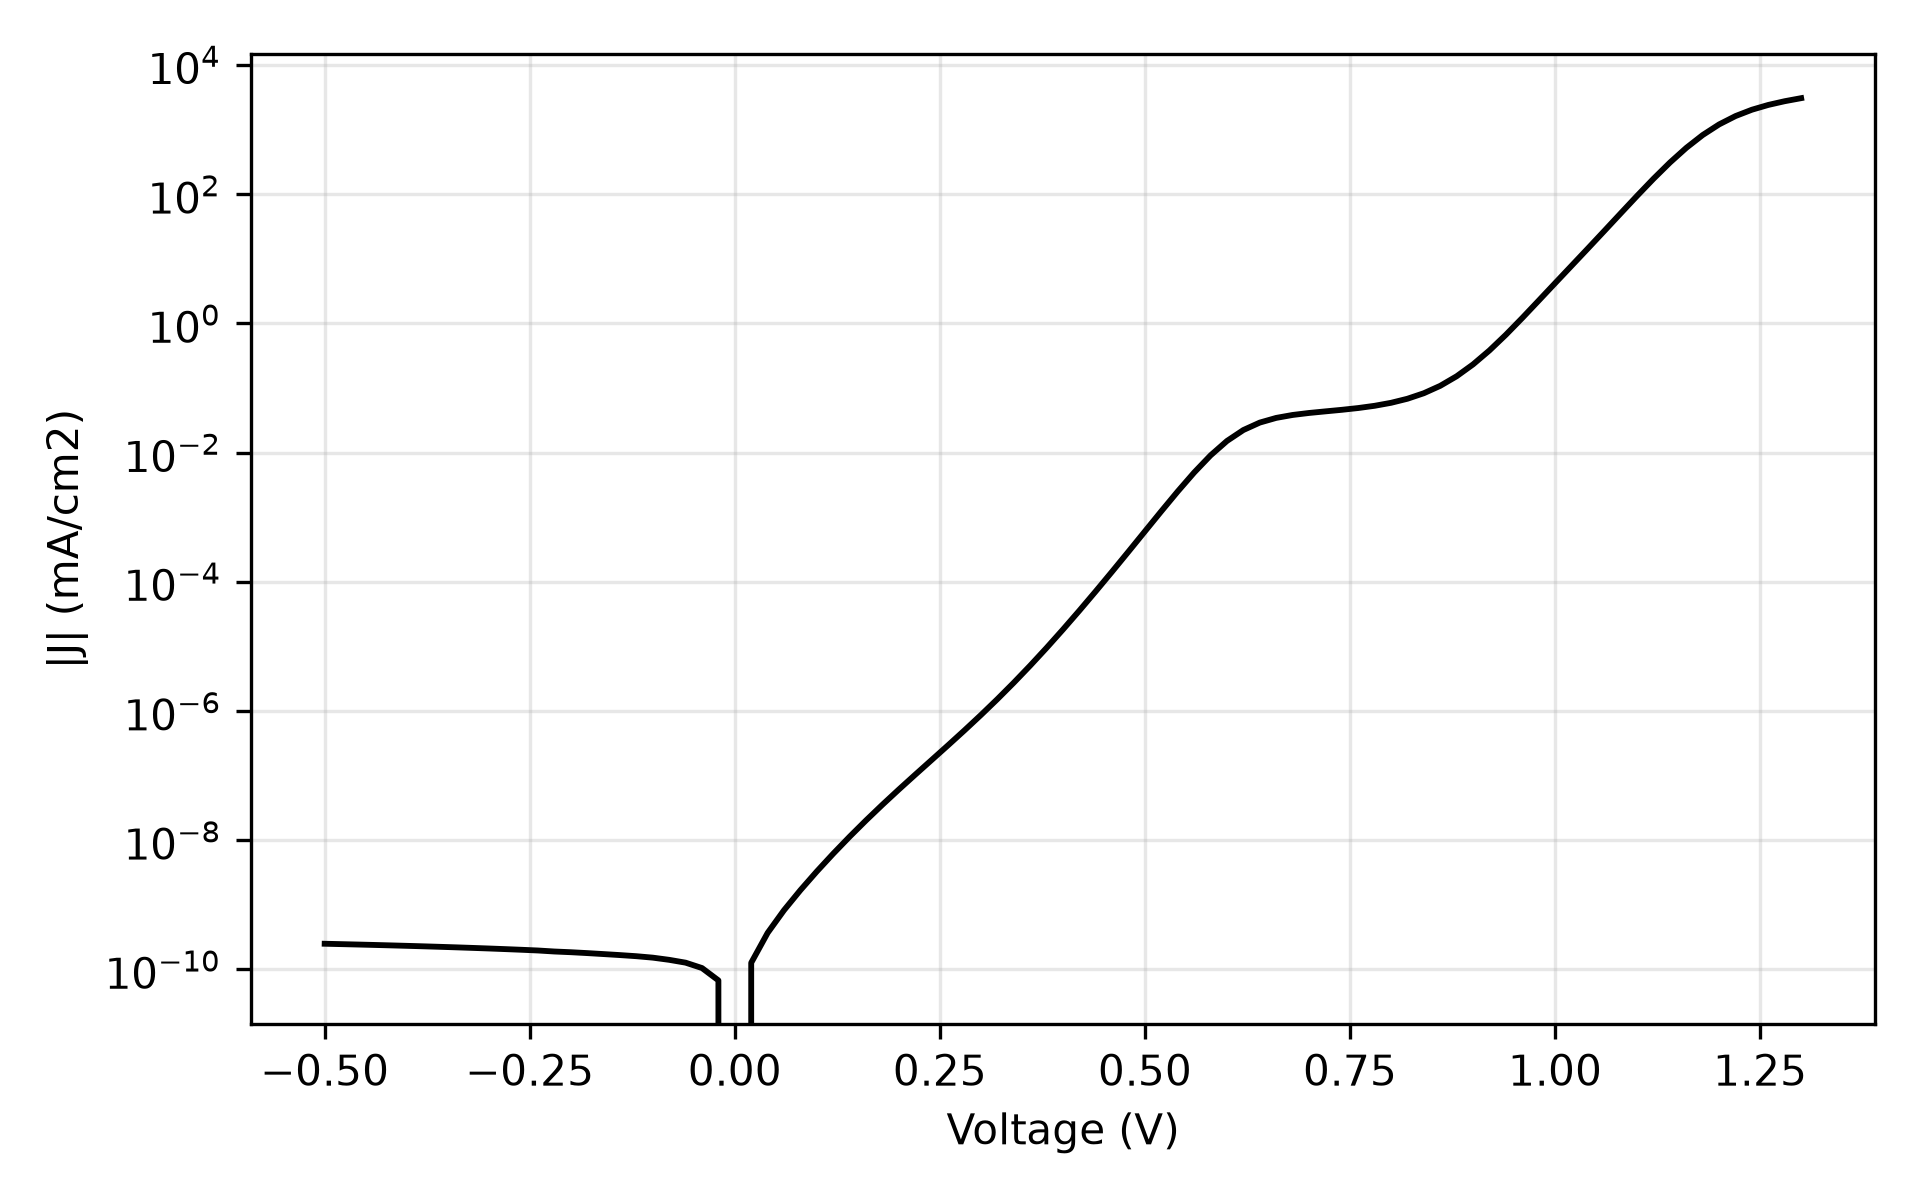
\includegraphics[width=0.85\linewidth]{figs/fig19.png}
\caption{Dark J--V characteristic of the optimized device. The forward branch is exponential over nearly three decades; the reverse branch remains below 10$^{-10}$ A/cm$^{2}$.}
\par\vspace{2pt}{\footnotesize\emph{Alt text: Semilogarithmic dark current-voltage curve with an exponential forward branch spanning nearly three decades and reverse leakage below ten to the minus-ten amperes per square centimetre.}}\par
\end{figure}

\section*{S3.\ Screening and simulation setup tables}
\begin{table}[htbp]
\centering
{\small\setlength{\tabcolsep}{3pt}
\begin{tabularx}{\textwidth}{XXcX}
\hline
Study (Year) [Ref.] & Device Structure & PCE (\%) & Key Limitation
\\\hline
Pindolia et al. (2022) \cite{r14} & FTO/\allowbreak{}TiO$_{2}$/RbGeI$_{3}$/NiO/\allowbreak{}Ag & 9.77 & Broad multi-parameter sweep (HTL, ETL, thickness, doping, defects, back contact, temperature); baseline efficiency remains modest and Ge$^{2+}$ oxidation not addressed.\\
Saikia et al. (2022) \cite{r24} & FTO/\allowbreak{}TiO$_{2}$/CsGeI$_{3}$/CuI/\allowbreak{}Au & 10.80 & No multi-HTL comparative analysis.\\
Bouazizi et al. (2022) \cite{r15} & FTO/\allowbreak{}PCBM/\allowbreak{}CsSn0.5Ge0.5I3/\allowbreak{}Spiro/Au & 18.13 & Mixed Ge/Sn absorber; thermal sensitivity.\\
Loumachi et al. (2024) \cite{r22} & ITO/\allowbreak{}C$_{60}$/RbGeI$_{3}$/CBTS/\allowbreak{}Ag & 27.21 & Optimized RbGeI$_{3}$ thickness and series/shunt resistance; interface defect optimization not addressed.\\
Raj et al. (2025) \cite{r39} & FTO/\allowbreak{}TiO$_{2}$/RbGeI$_{3}$/PEDOT:PSS/\allowbreak{}Au & 18.60 & Organic HTL limits long-term stability.\\
Pathak et al. (2026) \cite{r23} & FTO/\allowbreak{}TiO$_{2}$/RbGeI$_{3}$/Spiro-OMeTAD/\allowbreak{}Au & 26.47 & Ge$^{2+}$ $\rightarrow$ Ge$^{4+}$ oxidation not addressed; only single ETL/HTL combination studied.\\
Dash et al. (2025) \cite{r17} & DFT + SCAPS-1D of RbGeX$_{3}$ (X=Cl, Br, I) & 25.76 & Primarily material-level comparison; limited device-architecture optimization.\\
Samaki et al. (2023) \cite{r13} & FTO/\allowbreak{}TiO$_{2}$/RbGeI$_{3}$/Spiro/\allowbreak{}Ag & 18.10 & HTM screening that identified CuI; single-architecture optimization.\\
\hline
\end{tabularx}
}
\caption{Summary of recent SCAPS-1D studies on lead-free Ge-based and Sn-based perovskite solar cells.}
\par\vspace{2pt}{\footnotesize\emph{Alt text: Survey table listing eight recent simulations of germanium- and tin-based lead-free solar cells with device structure, efficiency and the key limitation of each study.}}\par
\end{table}
\begin{table}[htbp]
\centering
{\footnotesize\setlength{\tabcolsep}{3pt}
\begin{tabularx}{\textwidth}{Xcccc}
\hline
Parameter & TiO$_{2}$ & FTO & RbGeI$_{3}$ & CuI
\\\hline
Thickness (nm) & 30 & 500 & 400 & 100\\
Bandgap $E_{\mathrm{g}}$ (eV) & 3.2 & 3.2 & 1.4 & 3.1\\
Electron affinity $\chi$ (eV) & 4.0 & 4.4 & 3.9 & 2.1\\
Dielectric permittivity $\epsilon$r & 9 & 9 & 23.01 & 6.5\\
CB effective DOS N$_{\mathrm{C}}$ (cm$^{-3}$) & 2$\times$10$^{18}$ & 2.2$\times$10$^{18}$ & 1$\times$10$^{17}$ & 2.8$\times$10$^{19}$\\
VB effective DOS N$_{\mathrm{V}}$ (cm$^{-3}$) & 1.8$\times$10$^{19}$ & 1.8$\times$10$^{19}$ & 1$\times$10$^{17}$ & 1$\times$10$^{19}$\\
Electron mobility $\mu$e (cm$^{2}$ V$^{-1}$ s$^{-1}$) & 20 & 20 & 28.6 & 100\\
Hole mobility $\mu$p (cm$^{2}$ V$^{-1}$ s$^{-1}$) & 10 & 10 & 27.3 & 43.9\\
Donor density $N_{\mathrm{D}}$ (cm$^{-3}$) & 9$\times$10$^{16}$ & 1$\times$10$^{19}$ & 1$\times$10$^{9}$ & 0\\
Acceptor density $N_{\mathrm{A}}$ (cm$^{-3}$) & 0 & 0 & 1$\times$10$^{9}$ & 1$\times$10$^{18}$\\
Bulk defect density $N_{\mathrm{t}}$ (cm$^{-3}$) & 1$\times$10$^{15}$ & 1$\times$10$^{14}$ & 1$\times$10$^{15}$ & 1$\times$10$^{15}$\\
\hline
\end{tabularx}
}
\caption{Initial electrical and optical parameters used in the SCAPS-1D simulation of the proposed FTO/\allowbreak{}TiO$_{2}$/RbGeI$_{3}$/CuI/\allowbreak{}Au solar cell.}
\par\vspace{2pt}{\footnotesize\emph{Alt text: Parameter table giving thickness, bandgap, affinity, permittivity, densities of states, mobilities, doping and defect densities for the titanium oxide, fluorine-doped tin oxide, rubidium and copper-iodide layers.}}\par
\end{table}
\begin{table}[htbp]
\centering
{\small\setlength{\tabcolsep}{3pt}
\begin{tabularx}{\textwidth}{Xc}
\hline
Interface & Interface defect density $N_{\mathrm{t}}$ (cm$^{-2}$)
\\\hline
TiO$_{2}$ / RbGeI$_{3}$ & 1 $\times$ 10$^{14}$\\
RbGeI$_{3}$ / CuI & 1 $\times$ 10$^{14}$\\
\hline
\end{tabularx}
}
\caption{Initial interface defect density applied at each heterojunction.}
\par\vspace{2pt}{\footnotesize\emph{Alt text: Short table listing one ten-to-the-fourteenth per-square-centimetre defect densities applied at each of the two heterojunctions.}}\par
\end{table}
\begin{table}[htbp]
\centering
{\small\setlength{\tabcolsep}{3pt}
\begin{tabularx}{\textwidth}{XX}
\hline
Parameter & Value
\\\hline
Simulation software & SCAPS-1D version 3.3.10\\
Illumination spectrum & AM 1.5G\\
Incident power density & 100 mW/cm$^{2}$ (1000 W/m$^{2}$)\\
Operating temperature & 300 K (27 $^{\circ}$C)\\
Illumination intensity & 1 Sun\\
Scan mode & Illuminated J--V\\
Device type & Planar heterojunction\\
Front contact & FTO\\
Back contact & Au\\
Initial material parameters & Table S2\\
Initial interface defect density & Table S3\\
\hline
\end{tabularx}
}
\caption{Simulation conditions used in SCAPS-1D.}
\par\vspace{2pt}{\footnotesize\emph{Alt text: Key-value table of the simulation settings, including the solver version, the standard sunlight spectrum, one-sun intensity, room temperature and the front and back contact metals.}}\par
\end{table}
\begin{table}[htbp]
\centering
{\small\setlength{\tabcolsep}{3pt}
\begin{tabularx}{\textwidth}{Xccc}
\hline
BSF $d$ (nm) $\times$ $N_{A}$ (cm$^{-3}$) & $10^{17}$ & $10^{18}$ & $10^{19}$\\
\hline
30 & 27.55 & 27.93 & 28.00\\
50 & 27.59 & 27.93 & 28.00\\
80 & 27.60 & 27.94 & 28.01\\
100 & 27.60 & 27.94 & 28.01\\
\hline
\end{tabularx}}
\caption{BSF grid PCE (\%; \texttt{r8\_bsf.json}, 12/12 converged) on the rebased H1-adopted deck. Doping dominates; thickness flat within 0.01 pp at $N_{A}$ $10^{19}$ cm$^{-3}$.}
\par\vspace{2pt}{\footnotesize\emph{Alt text: Four-by-three grid of efficiency values over back-surface-field thickness and doping. Values rise with doping from about 27.6 to 28.0 percent while thickness has almost no effect.}}\par
\end{table}
\begin{table}[htbp]
\centering
{\small\setlength{\tabcolsep}{3pt}
\begin{tabularx}{\textwidth}{Xccc}
\hline
Waterfall node & $V_{\mathrm{OC}}$ (V) & $J_{\mathrm{SC}}$ (mA/cm$^{2}$) & PCE$_{1\text{-sun}}$ (\%)\\
\hline
H0 adopted (H1) & 1.0613 & 30.32 & 27.06\\
W1 +10\% reflection (90 mW/cm$^{2}$) & 1.0600 & 27.28 & 24.28\\
W2 +bulk $10^{15}$ cm$^{-3}$ (90 mW/cm$^{2}$) & 1.0200 & 27.28 & 21.93\\
S3 +interfaces $10^{15}$ cm$^{-2}$ (90 mW/cm$^{2}$) & 0.9800 & 27.27 & 20.78\\
S4 BSF on S3 stack (90 mW/cm$^{2}$) & 1.0100 & 27.27 & 21.76\\
\hline
\end{tabularx}}
\caption{Stacked loss waterfall (\texttt{r8\_waterfall\_JV.json} for W1/W2, \texttt{r8\_S3\_JV.json}, \texttt{r8\_s490\_JV.json}). Sub-1-sun points report PCE$_{1\text{-sun}}$ $=$ $VJ\mathrm{FF}/100$ explicitly since SCAPS normalizes \texttt{eta} to the set illumination.}
\par\vspace{2pt}{\footnotesize\emph{Alt text: Five-row table stepping the efficiency from the 27.06 percent ideal device through reflection, bulk and interface losses to 20.78 percent, recovering to 21.76 percent with the back-surface field.}}\par
\end{table}

\section*{S4.\ BSF, junction baseline and ML-surrogate notes}
\subsection*{BSF structure}
The BSF variant inserts a Cu$_{2}$O-like p$^{+}$ layer ($E_{\mathrm{g}}$ 2.1 eV, $\chi$ 3.2 eV, $\epsilon_{r}$ 7.5, $N_{A}$ $10^{17}$--$10^{19}$ cm$^{-3}$, 30--100 nm) between RbGeI$_{3}$ and CuI, splitting that interface into CuI/BSF and BSF/RbGeI$_{3}$, both carrying the same neutral-trap model as the interface they replace. BSF defs branch from the rebased H1-adopted deck, so the radiative correction is already in the base. Generating script: \texttt{r8\_bsf.py}; grid in \texttt{r8\_bsf.json}; ideal-BSF J--V in \texttt{r8\_BSF\_JV.json}; BSF-on-realistic-stack J--V in \texttt{r8\_s490\_JV.json}. Trap attribution runs (\texttt{r8\_DX\_*.def}, \texttt{r8\_DX\_a/b/c.json}): rear-$10^{16}$ on H1 gives 19.65\%; on BSF50-NA19 with both rear blocks raised gives 24.36\%, with only the absorber-side block raised also 24.36\%, and with only the far CuI/BSF block raised 28.00\% (no penalty). The p$^{+}$ no-offset control (BSF layer reset to CuI bands, $N_{A}$ kept) gives 27.82\% ideal and 21.33\% trapped.
\subsection*{Junction baseline}
Closed-form parameters anchored to the rebased H1 working point (scripted C--V capture returns header-only under v3.3.10 scripting, so no SCAPS C--V is claimed; $V_{\mathrm{bi}}$/depletion-width/Mott--Schottky claims are withdrawn since the near-intrinsic absorber is fully depleted): $n_{i}$ $1.75\times10^{12}$ m$^{-3}$ (from $N_{C}$=$N_{V}$ $10^{18}$ cm$^{-3}$, $E_{g}$ 1.4 eV); SRH $\tau$ 1000 ns at $10^{14}$ cm$^{-3}$; $L$ 8.6 $\mu$m $\gg$ 700 nm absorber; $\alpha$ $3.3\times10^{6}$ m$^{-1}$.
\subsection*{ML surrogate}
XGBoost/Random-Forest surrogates on the 200-point LHS-UQ block (8 features: $E_{g},N_{t},N_{C},N_{V},\mu_{n},\mu_{p},N_{\mathrm{int1}},N_{\mathrm{int2}}$, $\pm$25\% around the optimum, 80/20 split, seed 7): XGB R$^{2}$ 0.9074, RMSE 0.57; RF R$^{2}$ 0.9067. SHAP ranking: bulk $N_{t}$ $>$ $E_{g}$ $>$ $\mu_{n}$ $>$ CuI-side $N_{\mathrm{int2}}$ $>$ TiO$_{2}$-side $N_{\mathrm{int1}}$ $>$ $N_{V}$ $>$ $\mu_{p}$ $>$ $N_{C}$. Generating script: \texttt{r8\_ml.py}; metrics in \texttt{r8\_ml.json}; UQ block in \texttt{r8\_uq.json}.

\section*{S5.\ Experimental anchoring: methods and provenance}
\subsection*{Reference device}
Wang et al., Science 365, 591--595 (2019): FTO/c-TiO$_{2}$/$\beta$-CsPbI$_{3}$ (350--400 nm)/spiro-OMeTAD/Ag, AM1.5G, J--V at $\sim$45 $^{\circ}$C. Control 15.1\% (1.05 V, 20.03 mA/cm$^{2}$, 0.72); CHI-passivated champion 18.4\% (1.11 V, $\sim$20.0 mA/cm$^{2}$, 0.82); EQE-integrated J$_{\mathrm{SC}}$ 19.71/19.85 mA/cm$^{2}$; 32-device statistics.
\subsection*{Digitization}
Fig.~4A rendered at 400 dpi; tick-regression calibration ($\pm$0.002 V, $\pm$0.22 mA/cm$^{2}$); red/black color segmentation with blue-annotation and legend masking; column-median traces; legend-remnant filter. Self-check: extracted MPP metrics reproduce tabulated values within $\sim$1\% (control plateau reads $\sim$2\% low --- representative curve vs champion statistics, not fitted). CSVs: \url{validation/wang2019_ctrl_JV.csv}, \url{validation/wang2019_CHI_JV.csv}.
\subsection*{SCAPS rebuild}
Base: repo \texttt{perovskite-rbgei3.def}. Absorber $\rightarrow$ CsPbI$_{3}$ ($E_{g}$ 1.68 eV from UV-vis edge, $\chi$ 3.8, $\epsilon_{r}$ 10, $N_{C}$=$N_{V}$ $10^{19}$ cm$^{-3}$, $\mu$ 25/25 cm$^{2}$/Vs, 375 nm); HTL $\rightarrow$ doped spiro-OMeTAD ($\chi$ 2.3, $\mu$ $2\times10^{-3}$ cm$^{2}$/Vs for the Li-TFSI recipe, 180 nm); c-TiO$_{2}$ 40 nm; Ag back contact at effective 5.2 eV (pinned metal/organic interface; nominal 4.7 eV imposes a 0.5 eV barrier contradicted by the measured FF; 5.0/5.1 eV systematically fail to converge); sqrt-law $A=1.5\times10^{5}$ (Jsc-calibrated once); 318 K working point. Fitted: bulk $N_{t}$ $\times$ interface $N$ only. Champion: $3\times10^{13}$ cm$^{-3}$ / $3\times10^{13}$ cm$^{-2}$. Control: $3\times10^{13}$ cm$^{-3}$ / $10^{14}$ cm$^{-2}$ + external $V-JR_{s}$ correction $R_{s}=6.9$ $\Omega\cdot$cm$^{2}$ (defects alone floor FF at $\sim$0.84; cracks/pinholes/hysteresis documented). Builder: \url{validation/r7_validate.py}; grid: \url{validation/r7_grid_final.json}; best-fit J--V: \url{validation/r7_final_JV.json}; post-$R_{s}$ control J--V: \url{validation/r7_control_Rs69_JV.csv}; audit trail: \url{validation/VALIDATION_LOG.md} (includes non-converged runs).
\subsection*{Database benchmark}
Perovskite Database Project via NOMAD REST API, Oct.\ 2026: 43,106 \texttt{PerovskiteSolarCell} entries; 41,388 at 1-sun (600--1200 W/m$^{2}$); strict-inorganic filter (no MA/\allowbreak{}FA/\allowbreak{}BA/\allowbreak{}PEA/\allowbreak{}AVA/\allowbreak{}GU/\allowbreak{}NH$_{4}$/\allowbreak{}sulfonium/\allowbreak{}anilinium/\allowbreak{}thiocyanate tokens) $\rightarrow$ 2,201; archive-level J--V for all 2,201 (421 CsPbI$_{3}$). Analysis-clean counts used in the main text (41,316 one-sun, 2,141 inorganic) drop entries with missing or out-of-range metrics ($0<$ PCE $<35$, $0<V_{\mathrm{OC}}<2.5$, $0<$ FF $\le1$). Fetchers: \url{validation/nomad_fetch.py}, \url{validation/nomad_archives.py}; frozen cache: \url{validation/nomad_jv_clean.json}. Inorganic PCE: median 7.22\%, p90 13.74\%, max 18.22\%; CsPbI$_{3}$ max 17.82\%; 5 Ge-bearing entries (best 10.8\%), zero RbGeI$_{3}$.

\section*{S6.\ Oxidation-budget derivation and bounds}
Equilibrium V$_{\mathrm{Ge}}$ concentration $N=N_{\mathrm{sites}}\exp(-E^f/kT)$ with $N_{\mathrm{sites}}=1/a^3=4.87\times10^{21}$ cm$^{-3}$ ($a=5.9$~\AA) at 300~K gives: $E^f=0.46\rightarrow1.0\times10^{14}$; $0.40\rightarrow9.3\times10^{14}$; $0.35\rightarrow6.4\times10^{15}$; $0.30\rightarrow4.4\times10^{16}$; $0.15\rightarrow1.5\times10^{19}$~cm$^{-3}$. These land on the consolidated $N_t$ ladder (27.06/24.40/20.76\% at $10^{14}$/$10^{15}$/$10^{16}$ on the H1 deck) as plotted in main-text Fig.~24 (generator: \url{validation/r8_oxidation_fig.py}; case file: \url{validation/oxidation_case.md}). The 300~K values are lower bounds: freeze-in from 100~$^{\circ}$C (373~K) requires $E^f\approx0.57/0.50/0.42$~eV for $10^{14}$/$10^{15}$/$10^{16}$~cm$^{-3}$, and from 150~$^{\circ}$C (423~K) $0.65$/$0.56$/$0.48$~eV; processing bands in the main text are illustrative Ef assumptions. A current-state rung ($N_t=10^{17}$~cm$^{-3}$ on H1, \texttt{r8\_budget\_check.json}) gives 15.53\%. Tying doping to defects ($N_t=10^{15}$, $N_A=2\times10^{15}$~cm$^{-3}$) gives 25.52\% vs 24.40\% untied. Each V$_{\mathrm{Ge}}$ donates two holes, so $p\approx2$[V$_{\mathrm{Ge}}$] reproduces the $N_A$-collapse onset at $10^{16}$~cm$^{-3}$. SRH lifetimes $\tau^{-1}=\sigma v_{\mathrm{th}}N_t$ give 1000/100/10/1/0.1~ns at $N_t=10^{14}$--$10^{18}$~cm$^{-3}$; reported sub-ns TRPL in Ge-containing films \cite{rGeRev} therefore implies $N_t\gtrsim10^{17}$, 100--1000$\times$ above the $\le10^{15}$ tolerance. Bounds: energetics are CsGeI$_{3}$ DFT transferred to RbGeI$_{3}$ (same Ge--I framework; A-site band-edge-inert); equilibrium is a bound on kinetic oxidation; the V$_{I}$ deep-trap picture is functional-dependent, so no claim rests on V$_{I}$.

\section*{S7.\ Reproducibility appendix}
All SCAPS results were produced with SCAPS-1D v3.3.10 scripted through \texttt{scaps-runner} (\texttt{r5\_lib.py}: \texttt{BASE} deck, \texttt{run\_set}, \texttt{edit\_block}, \texttt{op\_summary\_only}). Base deck: repo \texttt{perovskite-rbgei3.def}; adopted deck: buildable as \texttt{r8\_H1\_adopted.def} (frozen in \texttt{REVIEW\_FIX\_LEDGER.md}). Run scripts and archives: OAT \texttt{r8\_oat.py} $\rightarrow$ \texttt{r8\_s*.json} + \texttt{r8\_oat\_summary.json}; extras/costs \texttt{r8\_extras.py} $\rightarrow$ \texttt{r8\_extras.json}; GA \texttt{r8\_ga.py} $\rightarrow$ \texttt{r8\_ga\_results.json} (best-found 28.30\% as optimizer reach below the adoption floors); BSF \texttt{r8\_bsf.py} $\rightarrow$ \texttt{r8\_bsf.json} (+$\epsilon_{r}$ extension \texttt{r8\_eps2.json}); trap-attribution and p$^{+}$-control runs $\rightarrow$ \texttt{r8\_DX\_a/b/c/d/e.json} (rear-only 20.29/19.65\%, front-only 13.12/10.77\%, both 10.59\% at $10^{15}$/$10^{16}$; far-side-only 28.00\%; p$^{+}$ control 27.82\% ideal, 21.33\% trapped; superseding the unattributed \texttt{r8\_nifsens.json} pair); D2 pipeline \texttt{r8\_D2.py} $\rightarrow$ \texttt{r8\_D2\_s\_*.json} + \texttt{r8\_D2\_chain.json} + \texttt{r8\_D2\_H1\_adopted.def} + \texttt{r8\_D2\_H1\_JV.json} (literature-standard NiO documented above, nothing fitted); stacked window \texttt{r8\_stack.py} $\rightarrow$ \texttt{r8\_stack.json} + \texttt{r8\_S3\_JV.json} + \texttt{r8\_s490\_JV.json}; optics waterfall nodes \texttt{r8\_waterfall\_JV.json} (W1 24.28\%, W2 21.93\%); temperature/Et/sigma/Cs \texttt{r8\_supplement.py} $\rightarrow$ \texttt{r8\_temp.json}, \texttt{r8\_etsigma.json}, \texttt{r8\_sigma.json}, \texttt{r8\_cs.json}; oxidation-budget checks \texttt{r8\_budget\_check.json} (current-state Nt17 rung 15.53\%, NA-tied Nt15 point 25.52\%); UQ/ML \texttt{r8\_uq.py}, \texttt{r8\_ml.py} $\rightarrow$ \texttt{r8\_uq.json}, \texttt{r8\_ml.json}; illumination/dark \texttt{r8\_darkillum.json}, \texttt{r8\_dark\_JV.json}. Known tooling limits, all disclosed in the main text: scripted \texttt{save results.qe} and \texttt{save results.cv} return header-only files under v3.3.10 scripting (no same-deck QE curve; no SCAPS C--V; junction claims withdrawn to lifetime-only); \texttt{save results.genrec} yields trap-occupation tables only. Non-convergent grid points (\texttt{r8\_s04\_chi\_3.7}, \texttt{r8x\_eg12}, D2 \texttt{chi\_3.7/4.2}) are reported as non-convergence, not omitted silently.texttt{r8\_bsf.json} (+$\epsilon_{r}$ extension \texttt{r8\_eps2.json}); trap-attribution and p$^{+}$-control runs $\rightarrow$ \texttt{r8\_DX\_a/b/c.json} (superseding the unattributed \texttt{r8\_nifsens.json} desensitization pair); stacked window \texttt{r8\_stack.py} $\rightarrow$ \texttt{r8\_stack.json} + \texttt{r8\_S3\_JV.json} + \texttt{r8\_s490\_JV.json}; optics waterfall nodes \texttt{r8\_waterfall\_JV.json} (W1 24.28\%, W2 21.93\%); temperature/Et/sigma/Cs \texttt{r8\_supplement.py} $\rightarrow$ \texttt{r8\_temp.json}, \texttt{r8\_etsigma.json}, \texttt{r8\_sigma.json}, \texttt{r8\_cs.json}; UQ/ML \texttt{r8\_uq.py}, \texttt{r8\_ml.py} $\rightarrow$ \texttt{r8\_uq.json}, \texttt{r8\_ml.json}; illumination/dark \texttt{r8\_darkillum.json}, \texttt{r8\_dark\_JV.json}; oxidation-budget checks \texttt{r8\_budget\_check.json} (current-state Nt17 rung, NA-tied Nt15 point). Known tooling limits, all disclosed in the main text: scripted \texttt{save results.qe} and \texttt{save results.cv} return header-only files under v3.3.10 scripting (no same-deck QE curve; no SCAPS C--V; junction claims withdrawn to lifetime-only); \texttt{save results.genrec} yields trap-occupation tables only; no GUI-automation tooling (\texttt{xdotool}/\texttt{wmctrl}/\texttt{pyautogui} absent) for scripted C--V. Non-convergent grid points (\texttt{r8\_s04\_chi\_3.7}, \texttt{r8x\_eg12}, D2 \texttt{chi\_3.7/4.2}) are reported as non-convergence, not omitted silently. The D2 NiO deck (\texttt{r8\_D2\_H1\_adopted.def}, script \texttt{r8\_D2.py}) substitutes literature-standard NiO ($E_{g}$ 3.6 eV, $\chi$ 1.8 eV, $\epsilon_{r}$ 11.7, $N_{C}$/$N_{V}$ $2.8\times10^{19}$/$10^{19}$ cm$^{-3}$, $\mu$ 12/2.8 cm$^{2}$/Vs, $N_{A}$ $10^{18}$ cm$^{-3}$) for CuI with the Au contact kept as in screening; nothing in it is fitted.

\begin{thebibliography}{99}
\bibitem{r13} S. Samaki et al., Sci.\ Rep.\ 13, 15517 (2023). doi:\url{10.1038/s41598-023-42471-w.}
\bibitem{r14} G. Pindolia et al., Sol.\ Energy 236, 802--821 (2022). doi:\url{10.1016/j.solener.2022.03.053.}
\bibitem{r15} S. Bouazizi et al., Mater.\ Res.\ Express 9(9), 096402 (2022). doi:\url{10.1088/2053-1591/ac8d52.}
\bibitem{r17} P. K. Dash et al., arXiv:2505.09362 (2025).
\bibitem{r22} L. Loumachi et al., East Eur.\ J.\ Phys.\ (3), 416--424 (2024). doi:\url{10.26565/2312-4334-2024-3-50}
\bibitem{r23} A. Pathak et al., Research Square (2026). doi:\url{10.21203/rs.3.rs-8749975/}
\bibitem{r24} D. Saikia et al., Opt.\ Mater.\ 123, 111839 (2022). doi:\url{10.1016/j.optmat.2021.111839.}
\bibitem{r39} M. Raj et al., J.\ Mater.\ Sci.\ 60(22), 9176--9196 (2025). doi:\url{10.1007/s10853-025-11002-5.}
\bibitem{r35} W. Shockley and H. J. Queisser, ``Detailed balance limit of efficiency of p-n junction solar cells,'' J. Appl. Phys. 32(3), 510--519 (1961). doi:\url{10.1063/1.1736034.}
\bibitem{r36} S. Rühle, ``Tabulated values of the Shockley--Queisser limit for single junction solar cells,'' Sol. Energy 130, 139--147 (2016). doi:\url{10.1016/j.solener.2016.02.015.}
\bibitem{r37} C. H. Henry, ``Limiting efficiencies of ideal single and multiple energy gap terrestrial solar cells,'' J. Appl. Phys. 51(8), 4494--4500 (1980). doi:\url{10.1063/1.328272.}
\bibitem{rGeRev} W. J. Jang, P. J. Park, W.-J. Ong and S. Y. Kim, ``Stable and eco-friendly inorganic lead-free perovskite solar cells: structural, electronic, and defect engineering,'' Commun.\ Mater.\ 7 (2026). doi:\url{10.1038/s43246-026-01158-1.}
\end{thebibliography}
\end{document}